\documentclass[11pt,fleqn]{article}
\usepackage{aip491}
\usepackage{graphicx} % Required for inserting images
% babel already loaded by aip491.sty with [vietnamese,main=english]
\usepackage{booktabs}
\usepackage{amsfonts,amsmath,amssymb}
\usepackage{siunitx}
\usepackage{multirow}
% aip491.sty only loads hyperref inside an \ifpdftex branch (i.e. only under
% pdflatex); load it here too if that branch was skipped (xelatex/lualatex),
% then set linktoc=all either way so every ToC line -- not just the page
% number -- is a clickable jump target.
\makeatletter
\@ifpackageloaded{hyperref}{}{\usepackage[hidelinks]{hyperref}}
\makeatother
\hypersetup{linktoc=all}
\usepackage{cleveref}

\usepackage{titlesec}
\usepackage{appendix}
\usepackage{algorithm}
\usepackage{algpseudocode}

\usepackage{comment}
\usepackage{placeins} % \FloatBarrier -- stops a figure/table from drifting
                       % past a section boundary into unrelated content
\newcommand{\sectionbreak}{}

% Loosen LaTeX's default float-placement limits so figures/tables with
% [htbp] don't queue up and get deferred to a pile at the end of the
% document -- allow more floats per page and more of the page to be
% covered by floats before forcing a dedicated float page.
\setcounter{topnumber}{4}
\setcounter{bottomnumber}{4}
\setcounter{totalnumber}{8}
\renewcommand{\topfraction}{0.9}
\renewcommand{\bottomfraction}{0.9}
\renewcommand{\textfraction}{0.05}
\renewcommand{\floatpagefraction}{0.75}

% Show every heading level (section / subsection / subsubsection / paragraph) in the
% numbering and in the Table of Contents, so the ToC reflects the full outline.
\setcounter{secnumdepth}{4}
\setcounter{tocdepth}{4}

\advisor{Nguyen Xuan Huy}
\coadvisor{Nguyen Quoc Trung}
\gpname{GSU05}
\cpcode{SU26AI48\_GSU05}
\gmemf{Lê Hoàng Nam - Member - SE180304}
\gmemsc{Lâm Vương - Member - SE184202}
\gmemth{Đào Quang Minh - Member - SE184321}
\gmemfo{Trần Bá Thành - Member - HE171047}
\gmemnS{4}  % Number of students in group, should be 3 or 4

\title{Adaptive Layered Quantum \\ Neural Networks (AL-QNN) \\ for Mitigating Barren Plateaus \\ in NISQ Devices}  % Project title
\graduateDate{HCMC, Aug 2026}

\begin{document}

\pagestyle{empty}
\maketitle
\pagestyle{plain}

\pagenumbering{arabic}
\setstretch{1.08} %\doublespacing  %

\tableofcontents

\cleardoublepage
\addcontentsline{toc}{section}{\listfigurename}
\listoffigures
\cleardoublepage
\addcontentsline{toc}{section}{\listtablename}
\listoftables
\cleardoublepage

\section*{Acknowledgement}
\addcontentsline{toc}{section}{Acknowledgement}
We would like to thank our supervisors, Nguyen Xuan Huy and Nguyen Quoc Trung, for their guidance throughout
the project, from framing the barren-plateau problem to reviewing the experimental methodology and results.
Their willingness to question early, overconfident claims and to insist on multi-seed evidence before any
scheduler was declared successful shaped the data-honesty principle that runs through this entire report.

We are also grateful to the Department of Artificial Intelligence at FPT University for the computing
resources and coursework structure that made this capstone possible, and to the members of the GSU05
capstone group -- Lê Hoàng Nam, Lâm Vương, Đào Quang Minh, and Trần Bá Thành -- whose complementary work
on the variational model, the reinforcement-learning scheduler, the dataset pipeline, and the project's
documentation each made the others' work possible. We would further like to thank our peers and the
committee members who reviewed earlier stages of this work and whose questions repeatedly sent us back
to the logs to check a claim before we were willing to write it down.

Finally, we thank our families and friends for their patience and support during the months of
experimentation, debugging, and writing that went into this report.

\clearpage
\section*{Definitions and Acronyms}
\addcontentsline{toc}{section}{Definitions and Acronyms}
\begin{table}[htbp]
\centering
\caption{Definitions and acronyms.}
\label{tab:acronyms}
\begin{tabular}{|p{3cm}|p{11cm}|}
\hline
\textbf{Acronym} & \textbf{Definition} \\
\hline
AL-QNN & Adaptive Layered Quantum Neural Network -- a variational quantum circuit whose depth is scheduled online by a reinforcement-learning agent. \\
\hline
VQC & Variational Quantum Classifier -- a parameterized quantum circuit trained to classify data. \\
\hline
VQE & Variational Quantum Eigensolver -- a variational algorithm that estimates the ground-state energy of a Hamiltonian, discussed in Section~3 as background for barren-plateau mitigation strategies that carry over to VQC. \\
\hline
HEA & Hardware-Efficient Ansatz -- layers of single-qubit rotations followed by fixed entangling gates. \\
\hline
MDP & Markov Decision Process -- the formal (S, A, P, R, $\gamma$) framework used to model the depth scheduler (Section~4.7.2). \\
\hline
Barren Plateau (BP) & A regime where the variance of the cost gradient vanishes with the number of qubits and/or circuit depth, making gradient-based training infeasible. \\
\hline
PCA & Principal Component Analysis -- dimensionality reduction used to fit features to the qubit count. \\
\hline
PennyLane & Quantum machine-learning library used as the statevector simulator for deployment (Section~4.7.1). \\
\hline
NISQ & Noisy Intermediate-Scale Quantum -- the current generation of quantum hardware with limited qubits and no error correction. \\
\hline
Angle encoding & Feature map that loads a classical value into a qubit rotation angle. \\
\hline
RL & Reinforcement Learning. \\
\hline
PPO / DQN & Proximal Policy Optimization / Deep Q-Network -- the two RL algorithms used for the scheduler. \\
\hline
ROC AUC & Area under the Receiver Operating Characteristic curve -- reported as an explicit column in the fixed-depth sweep tables of Section~6.2, and cited for individual scheduler runs throughout the discussion in Section~6.1. \\
\hline
\end{tabular}
\end{table}

\clearpage

\section{Project Introduction}
\subsection{Overview}
This report documents the design, implementation, and evaluation of AL-QNN, a variational quantum classifier whose circuit depth is adjusted online by a reinforcement-learning agent in order to keep the model trainable in the presence of barren plateaus. Section~2 describes the project management plan. Section~3 reviews the state of the art in quantum machine learning and barren-plateau mitigation. Section~4 details the reinforcement-learning methodology. Section~5 presents the system design and implementation. Section~6 reports and discusses the results across several backends and cost regimes, with particular attention to when adaptive scheduling helps and when it does not. Section~7 concludes and outlines future work.

\subsection{Background and Motivation}
Variational quantum algorithms are among the most promising candidates for demonstrating practical value on today's Noisy Intermediate-Scale Quantum (NISQ) hardware. They combine a parameterized quantum circuit with a classical optimizer, so that the quantum device only has to execute shallow circuits while the heavy optimization runs classically. However, a fundamental obstacle stands in the way: the barren-plateau phenomenon. As the number of qubits grows, the variance of the cost-function gradient vanishes exponentially, so the optimizer receives essentially no signal and training stalls.

A natural but naive response is to fix the circuit depth in advance. This fails in both directions: a circuit that is too shallow cannot express the target function (underfitting), while a circuit that is too deep sinks deeper into the barren-plateau region and becomes untrainable. Choosing the right depth by hand for every dataset and qubit count is impractical. This project asks whether a reinforcement-learning agent can instead schedule the depth online -- adding capacity when gradients are healthy and pruning it when they are not -- using live telemetry from the circuit itself.

This question sits at the intersection of two active research programs. On the quantum side, the community has largely treated barren plateaus as a property to be measured and, where possible, avoided by construction -- through initialization strategies, restricted ansatz families, or problem-inspired circuit designs (Section~3). Comparatively little work treats the plateau as something to be actively managed at training time by an agent that observes it directly. On the machine-learning side, reinforcement learning has repeatedly proven effective at exactly this kind of online resource-allocation problem -- deciding, step by step, how much capacity or compute to commit to a task based on live feedback -- in domains from neural architecture search to robotics. AL-QNN sits at the overlap: it applies an RL formulation, otherwise unremarkable, to a resource-allocation decision (circuit depth) that is unremarkable in machine learning generally but has a genuinely quantum-specific failure mode (the barren plateau) driving it.

A further practical motivation is that near-term quantum devices are themselves resource-constrained: circuit depth is not a free parameter even ignoring trainability, because deeper circuits accumulate more gate error and take longer to execute on real hardware. A scheduler that commits to the shallowest depth sufficient for a given dataset and cost regime is therefore not only a trainability aid but also, in principle, a resource-efficiency mechanism -- a secondary benefit that this project does not evaluate directly (Section~1.6) but that motivates why depth, specifically, rather than some other circuit hyperparameter, was chosen as the control variable.

\subsection{Project Objective}
The high-level objective is to build and evaluate an RL agent that adaptively schedules the depth of a hardware-efficient variational circuit so as to maintain trainable gradients while achieving competitive classification performance. Concretely, the project aims to:

\begin{itemize}
\item Characterize the barren-plateau regime empirically as a function of qubit count and circuit depth on real datasets.
\item Design a Markov Decision Process in which an agent observes circuit telemetry and chooses to add, prune, or hold layers.
\item Train PPO and DQN agents efficiently using a fast classical surrogate, then deploy the learned policy on a PennyLane statevector simulator.
\item Evaluate the scheduler against static baselines (a hand-tuned rule and a greedy heuristic) across several regimes, and honestly characterize the conditions under which adaptive scheduling provides an advantage.
\end{itemize}

\subsection{Problem Statement}
Formally, training a variational quantum circuit means minimizing a cost function $C(\theta)$ over the circuit parameters $\theta$. Under a global cost and a sufficiently expressive ansatz, the gradient variance $\mathrm{Var}[\partial C/\partial\theta]$ decays as $O(2^{-n})$ in the qubit count $n$ \citep{mcclean2018barren}; this is the barren plateau. In this regime the optimizer's updates are dominated by shot noise and the loss does not decrease. The severity also depends on the cost definition: a local cost weakens the plateau but introduces a dependence on circuit depth \citep{cerezo2021cost}, so depth becomes a genuine control variable rather than a free parameter.

\begin{figure}[htbp]
\centering
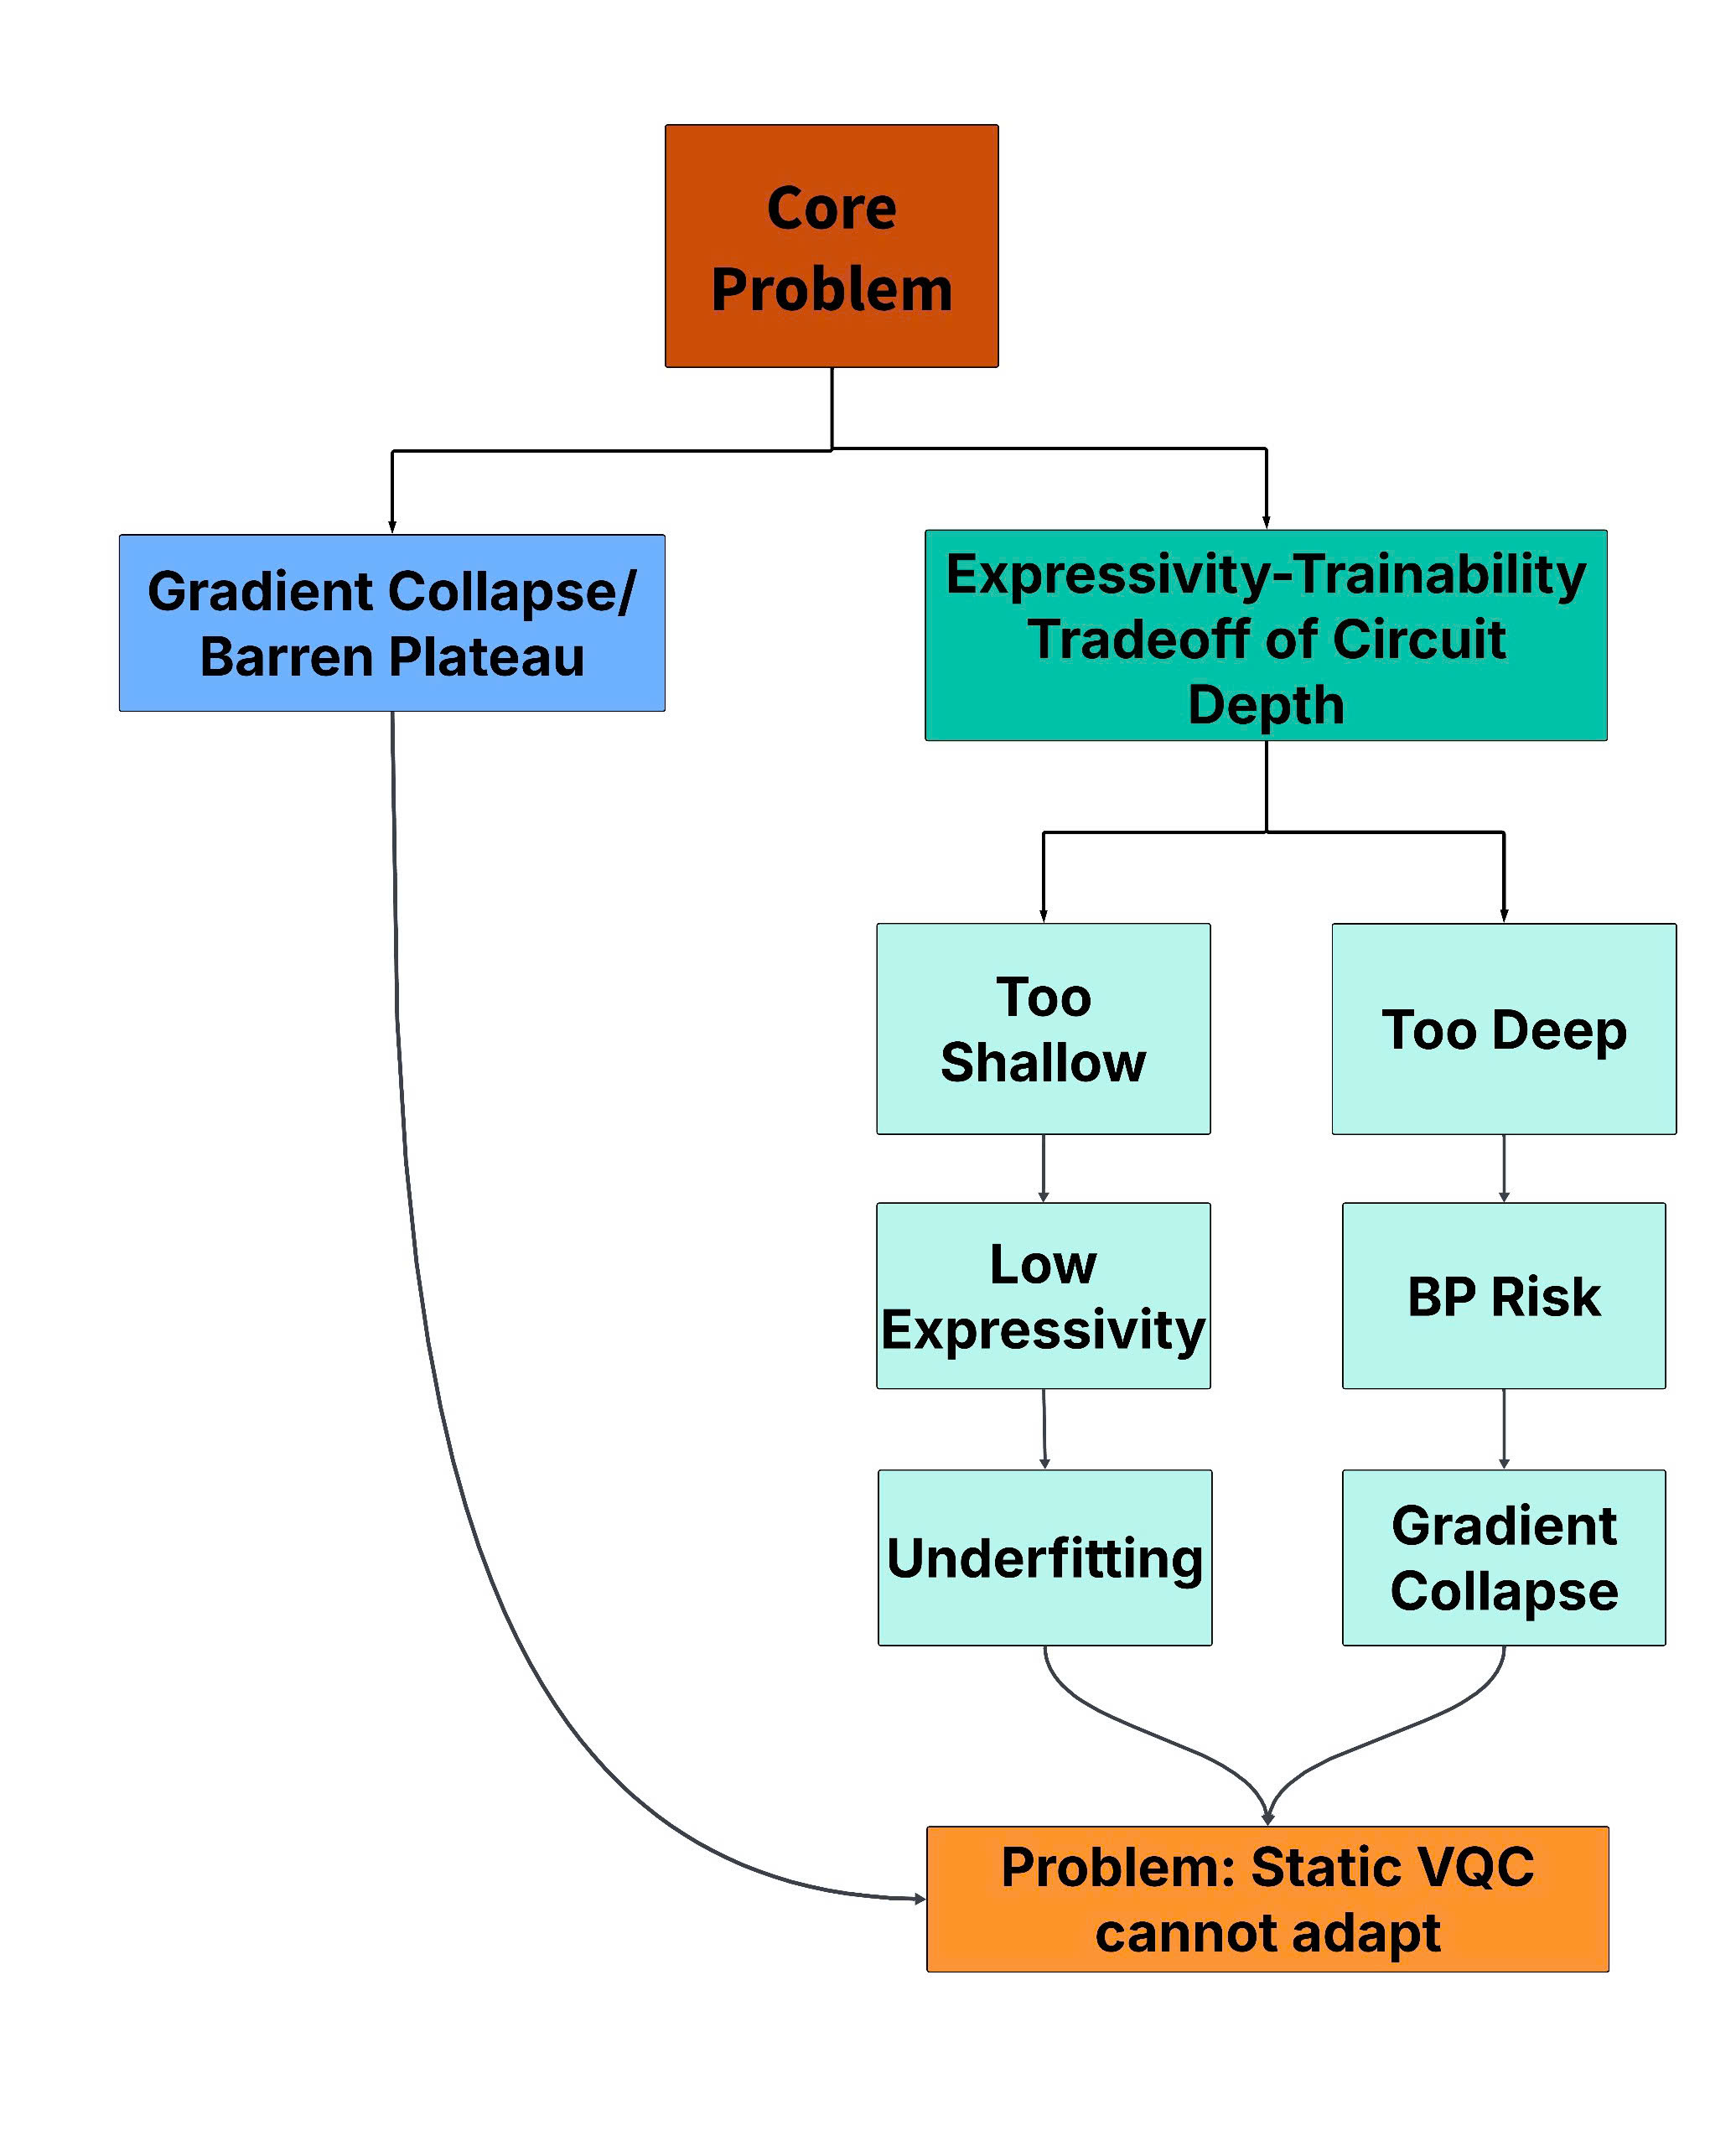
\includegraphics[width=0.75\textwidth]{figure/fig_problem_framing.jpg}
\caption{Problem framing. A fixed circuit depth fails in both directions: too shallow gives low expressivity and underfitting; too deep raises barren-plateau risk and gradient collapse. Both paths, together with the separate qubit-count-driven barren-plateau mechanism, converge on the same obstacle -- a static VQC cannot adapt to what the data and the current training state actually require.}
\label{fig:problem_framing}
\end{figure}

The engineering problem is therefore twofold. First, the depth of the circuit must be chosen adaptively, because the correct depth depends on the dataset, the qubit count, and the cost type, none of which are known a priori. Second, any adaptation must be driven by information that is actually observable during training -- gradient magnitudes, loss dynamics, and near-zero-gradient ratios -- rather than by an oracle. The project addresses both by casting depth scheduling as a reinforcement-learning problem over circuit telemetry.

A third, more subtle requirement follows from the first two: because the correct depth is regime-dependent rather than universal, any claim that a given scheduler is ``better'' is only meaningful relative to a specific dataset, qubit count, and cost type. A scheduler that wins in one regime may lose in another, and an evaluation methodology that reports results from only one regime risks presenting a partial, misleadingly general picture. This is why Section~6 deliberately reports results across several regimes (one real deployment and a synthetic comparison isolating cost type, all at the qubit counts validated on available hardware) rather than a single headline number: the project's empirical contribution is as much about characterizing the boundary of where adaptive scheduling helps as it is about the scheduler itself. Section~6.1 additionally reports three supplementary single-seed real deployments on other datasets (German Credit, Parkinson's, Pima); these sit outside the core evaluation design and are not weighted as evenly as the core regimes, but they were already available from the project's data-preparation work and are reported for completeness rather than left undocumented.

\subsection{Significance of the Project}
The theoretical contribution is a principled, telemetry-driven formulation of circuit-depth scheduling as an MDP, together with an honest empirical characterization of the regime in which reinforcement learning improves on simple static baselines. Rather than claiming universal superiority, the project identifies the specific conditions -- principally a local cost, where the plateau is depth-dependent rather than fixed -- under which adaptive scheduling separates from static schedulers. This nuanced result is itself a useful finding for practitioners.

The practical contribution is a reusable two-simulator architecture that makes RL training tractable for quantum circuits: a fast classical surrogate for the millions of environment steps required by RL, and a PennyLane statevector backend for faithful deployment and evaluation. The same pipeline is demonstrated on a real deployment (Heart Disease) and on a synthetic comparison isolating cost type.

\subsection{Scope and Limitations}
\textbf{Scope.} The project covers binary classification with hardware-efficient variational circuits, at up to 8 qubits on real datasets; evaluation runs on a statevector simulator (PennyLane) and on a calibrated classical surrogate (Section~4.7.1). The 8-qubit ceiling is a hardware limitation, not a design choice: PennyLane's statevector simulation and the RL deployment loop built on top of it become impractically slow and memory-hungry on the team's available machines beyond this range, so larger qubit counts were not pursued for the results reported here. The reinforcement-learning agent schedules circuit depth (add/prune/hold) and entanglement adjustments, trained with PPO and DQN. Preprocessing, barren-plateau measurement, deployment, and a demonstration interface are all included.

\textbf{Limitations.} Results are obtained on a noiseless statevector simulator, not on physical NISQ hardware; hardware noise is out of scope. The 8-qubit ceiling (above) means the barren-plateau scaling and the primary AI4I benchmark, both of which need a wider qubit range to show a strong effect, are correspondingly modest; AI4I was used with three seeds during development to characterize seed variance, and the scheduler-comparison tables presented in Section~6 are single-seed across datasets, backends, and cost regimes, and are labelled as exploratory.


\section{Project Management Plan}
\subsection{Team Work}
\subsubsection{Team Structure and Roles}
The team has no single team leader; responsibility is instead distributed across the five approaches that make up AL-QNN's methodology (Section~4.4), with overlapping support where two approaches are closely coupled. This report is authored from the perspective of the reinforcement-learning module (Approach~4--5).

\begin{table}[htbp]
\centering
\caption{Team structure and roles.}
\label{tab:team}
\begin{tabular}{|p{3.2cm}|p{10cm}|}
\hline
\textbf{Member} & \textbf{Responsibility} \\
\hline
Lâm Vương & Approach~4--5: the RL scheduler (PPO/DQN) and the computational two-simulator design (calibrated surrogate, PennyLane deployment); environment and telemetry integration. \\
Lê Hoàng Nam & Approach~2--3: adaptive circuit scheduling (hardware-efficient ansatz, action space) and safe mutation (soft-masking, commit/rollback registry); barren-plateau measurement (Stage 1B/1C). \\
Đào Quang Minh & Dataset acquisition, preparation, and visualization; supports the Rule and Greedy static baseline schedulers. \\
Trần Bá Thành & Approach~1: multi-dimensional gradient telemetry and diagnosis; supports Lê Hoàng Nam on Approach~2--3. \\
\hline
\end{tabular}
\end{table}

\quad \textbf{Supervisors:} Nguyen Xuan Huy; Nguyen Quoc Trung

\subsubsection{Communication Plan}
The team held weekly progress meetings with the supervisors and communicated daily through a group chat channel. Source code and experimental results were shared through a common repository, and every reported number was required to trace back to a committed CSV log, so that results could be independently re-checked by any team member or advisor.

\begin{itemize}
\item Weekly advisor meeting: progress against the WBS, blockers, and sign-off on any change to the ansatz, reward weights, or evaluation protocol before it was adopted project-wide.
\item Daily internal check-in: short async updates on which stage each member was working on, surfaced early when the RL module (Section~4.7) needed a specific telemetry field from the VQC module (Section~4.4.2) before it could proceed.
\item Shared repository as the single source of truth: every deployment log, comparison table, and figure referenced in this report resolves to a specific committed file (Appendix~D), which is what made the cross-checking practice in the paragraph above enforceable rather than aspirational.
\end{itemize}

\subsubsection{Tools and Repository}
The team used a single shared Git repository for all code, with the quantum-circuit and preprocessing code under the ownership of the VQC-side members and the environment, agent, and deployment code under the ownership of the RL-side member (\Cref{tab:team}). Experimental configuration -- dataset, qubit count, cost type, and backend -- was passed as explicit command-line arguments to the training and comparison scripts listed in Appendix~C, rather than hard-coded, so that a given experiment could be reproduced or varied along a single axis without touching the underlying code. This convention is what made the qubit-count and cost-type sweep reported in Section~6 practical to run as a set of independent, differently-configured invocations of the same two scripts.

\subsection{Project Management Approach}
\subsubsection{Work Breakdown Structure (WBS)}
\begin{table}[htbp]
\centering
\caption{Work breakdown structure (WBS).}
\label{tab:wbs}
\begin{tabular}{|p{2cm}|p{8cm}|p{3.5cm}|}
\hline
\textbf{Phase} & \textbf{Task} & \textbf{Owner} \\
\hline
Stage 1 & Barren-plateau characterization: gradient-variance measurement vs qubits and depth. & Lê Hoàng Nam \\
Stage 1C & Surrogate calibration: fit loss-floor and gradient-variance curves from measured data. & Lâm Vương, Lê Hoàng Nam \\
Stage 2 & RL environment: MDP, telemetry engine, mutation engine, reward. & Lâm Vương \\
Stage 2 & Agent training: PPO and DQN on the surrogate. & Lâm Vương \\
Stage 3 & Deployment: run learned policy on PennyLane; compare against rule and greedy. & Đào Quang Minh \\
Stage 3 & Extended fixed-depth sweep and cost-type regime comparison at the project's 8-qubit scope (Section~6.1--6.2). & Đào Quang Minh, Lâm Vương \\
Rework & Ansatz change (RX-RY-RZ to RZ-RY-RZ) and surrogate re-calibration (Section~2.2.4). & Lê Hoàng Nam, Lâm Vương \\
Rework & Preprocessing standardization: fit-on-train, Z-score before PCA (Section~2.2.4). & Lê Hoàng Nam \\
Support & Datasets, preprocessing pipeline, visualization, demo. & Lê Hoàng Nam, Đào Quang Minh, Lâm Vương \\
Support & Results logging and report documentation. & Trần Bá Thành \\
Exploratory & Telemetry ablation study (with versus without telemetry guardrails, Section~6.1). & Lâm Vương \\
\hline
\end{tabular}
\end{table}

\subsubsection{Risk Management}
\begin{table}[htbp]
\centering
\caption{Risk register.}
\label{tab:risk}
\begin{tabular}{|p{5cm}|p{2.5cm}|p{6.5cm}|}
\hline
\textbf{Risk} & \textbf{Impact} & \textbf{Mitigation} \\
\hline
PennyLane too slow for RL training (millions of steps). & Training infeasible. & Two-simulator design: train on a fast classical surrogate, deploy on PennyLane. \\
Single-seed results are unstable. & Overclaiming. & Report the primary dataset with three seeds; label single-seed results as exploratory. \\
Surrogate diverges from the real circuit after an ansatz change. & Sim-to-real gap. & Re-calibrate the surrogate whenever the ansatz or preprocessing changes. \\
A single fixed-depth sweep on one seed is read as a precise accuracy-vs-depth curve. & Overclaiming a scheduler advantage that is really sampling noise. & Report the sweep as illustrative (Section~6.2) and flag any non-monotonic point explicitly rather than smoothing over it. \\
Data leakage between preprocessing splits. & Inflated accuracy that would not replicate. & Fit every scaler and PCA transform on the training split only, enforced as a single shared preprocessing function (Section~4.2). \\
\hline
\end{tabular}
\end{table}

\subsubsection{Quality Management}
Quality was enforced through three practices. First, data honesty: every figure in this report is intended to trace to a real CSV log produced by the deployment pipeline, and claims that could not be substantiated by logs were removed; one table's original per-seed logs were later found to be unlocatable in the repository, and that gap is disclosed explicitly rather than hidden (Appendix~A.0). Second, a single-source-of-truth code structure: the hardware-efficient ansatz is defined exactly once, so a change there propagates consistently to every stage. Third, multi-seed evaluation on the primary dataset, with explicit caveats wherever only a single seed was available.

\subsubsection{Change Management Process}
Two significant changes occurred during the project and were handled explicitly. The variational ansatz was changed from an RX-RY-RZ rotation block to an RZ-RY-RZ (Euler Z-Y-Z) block; because this preserves three parameters per qubit, parameter counts were unchanged, but the surrogate calibration was scheduled for re-run. The preprocessing pipeline was standardized to fit all scalers on the training split only and to apply a Z-score standardization before PCA, preventing large-scale features from dominating the principal components.

\subsubsection{Closure and Evaluation}
The project closes with a committee defense and this final report. Lessons learned -- particularly the importance of multi-seed evaluation and of honestly reporting cases where the learned agent does not beat a simple baseline -- are captured in the discussion and conclusion.


\section{Literature Review}
\quad This chapter surveys the theoretical and technological foundations underpinning our research: variational quantum algorithms, the barren-plateau phenomenon and its causes, existing static and heuristic mitigation strategies, and the use of reinforcement learning in scientific and quantum control problems. We position AL-QNN within this landscape and identify the specific gap it addresses.

\subsection{Overview of the Field}
Quantum machine learning studies how parameterized quantum circuits can represent and learn functions of classical or quantum data. In the variational paradigm, a circuit U($\theta$) prepares a state whose measurement defines a model output; the parameters $\theta$ are optimized classically. The central open problem for these models is trainability, dominated by the barren-plateau phenomenon.

\subsubsection{Variational Quantum Circuits and the Hardware-Efficient Ansatz}
On NISQ hardware, the hardware-efficient ansatz -- alternating layers of single-qubit rotations and fixed entangling gates -- is popular because it respects device connectivity and keeps circuits shallow.

\subsubsection{VQE and VQC: Two Families of Variational Algorithms}
Two broad families of variational algorithm dominate the field. The first, exemplified by the Variational Quantum Eigensolver (VQE), targets physics and chemistry problems where the cost function is the expectation value of a Hamiltonian and the goal is to find its ground-state energy. The second, exemplified by the Variational Quantum Classifier (VQC) used in this project, targets supervised learning problems where the cost function is a classification loss computed from measurement outcomes on labelled data. The two families share the same underlying machinery -- a parameterized circuit, a classical optimizer, and a scalar cost evaluated via measurement -- and, as a consequence, share the same trainability pathology. This is why barren-plateau mitigation strategies developed for VQE chemistry problems, such as ADAPT-VQE, are directly relevant background for a VQC depth-scheduling project even though the target application domains differ.

\subsubsection{Data Encoding Strategies}
A separate but related question is how the classical data enters the circuit in the first place. This project uses angle encoding, where each classical feature is loaded as the rotation angle of a single-qubit gate; this is simple, hardware-efficient, and keeps the encoding circuit shallow, at the cost of requiring one qubit per feature (hence the feature-count-to-qubit-count matching described in Section~4.3). Denser encodings, such as amplitude encoding, can represent exponentially more features per qubit but require circuits that are themselves harder to prepare and differentiate reliably on near-term hardware, which is why angle encoding remains the standard choice for hardware-efficient classifiers of the kind studied here.

\subsection{Historical Context}

\subsubsection{Origins of Variational Quantum Algorithms}
Variational quantum algorithms were introduced with the Variational Quantum Eigensolver of \citet{peruzzo2014variational} and popularized for machine learning by the hardware-efficient ansatz of \citet{kandala2017hardware}.

\subsubsection{Discovery and Refinement of the Barren-Plateau Phenomenon}
The barren-plateau phenomenon was identified by \citet{mcclean2018barren}, who showed that for sufficiently random deep circuits the gradient variance decays exponentially with the qubit count. Subsequent work by \citet{cerezo2021cost} refined this picture, showing that local cost functions exhibit weaker, depth-dependent plateaus, which is precisely the regime this project exploits. Between these two results, the field's understanding of the barren plateau shifted from a qubit-count phenomenon alone to a joint function of qubit count, circuit depth, ansatz expressivity, and the locality of the cost -- a four-factor picture that motivates treating depth as a controllable variable rather than a fixed hyperparameter, which is the starting point for this project's MDP formulation in Section~4.7.2.

\begin{figure}[htbp]
\centering
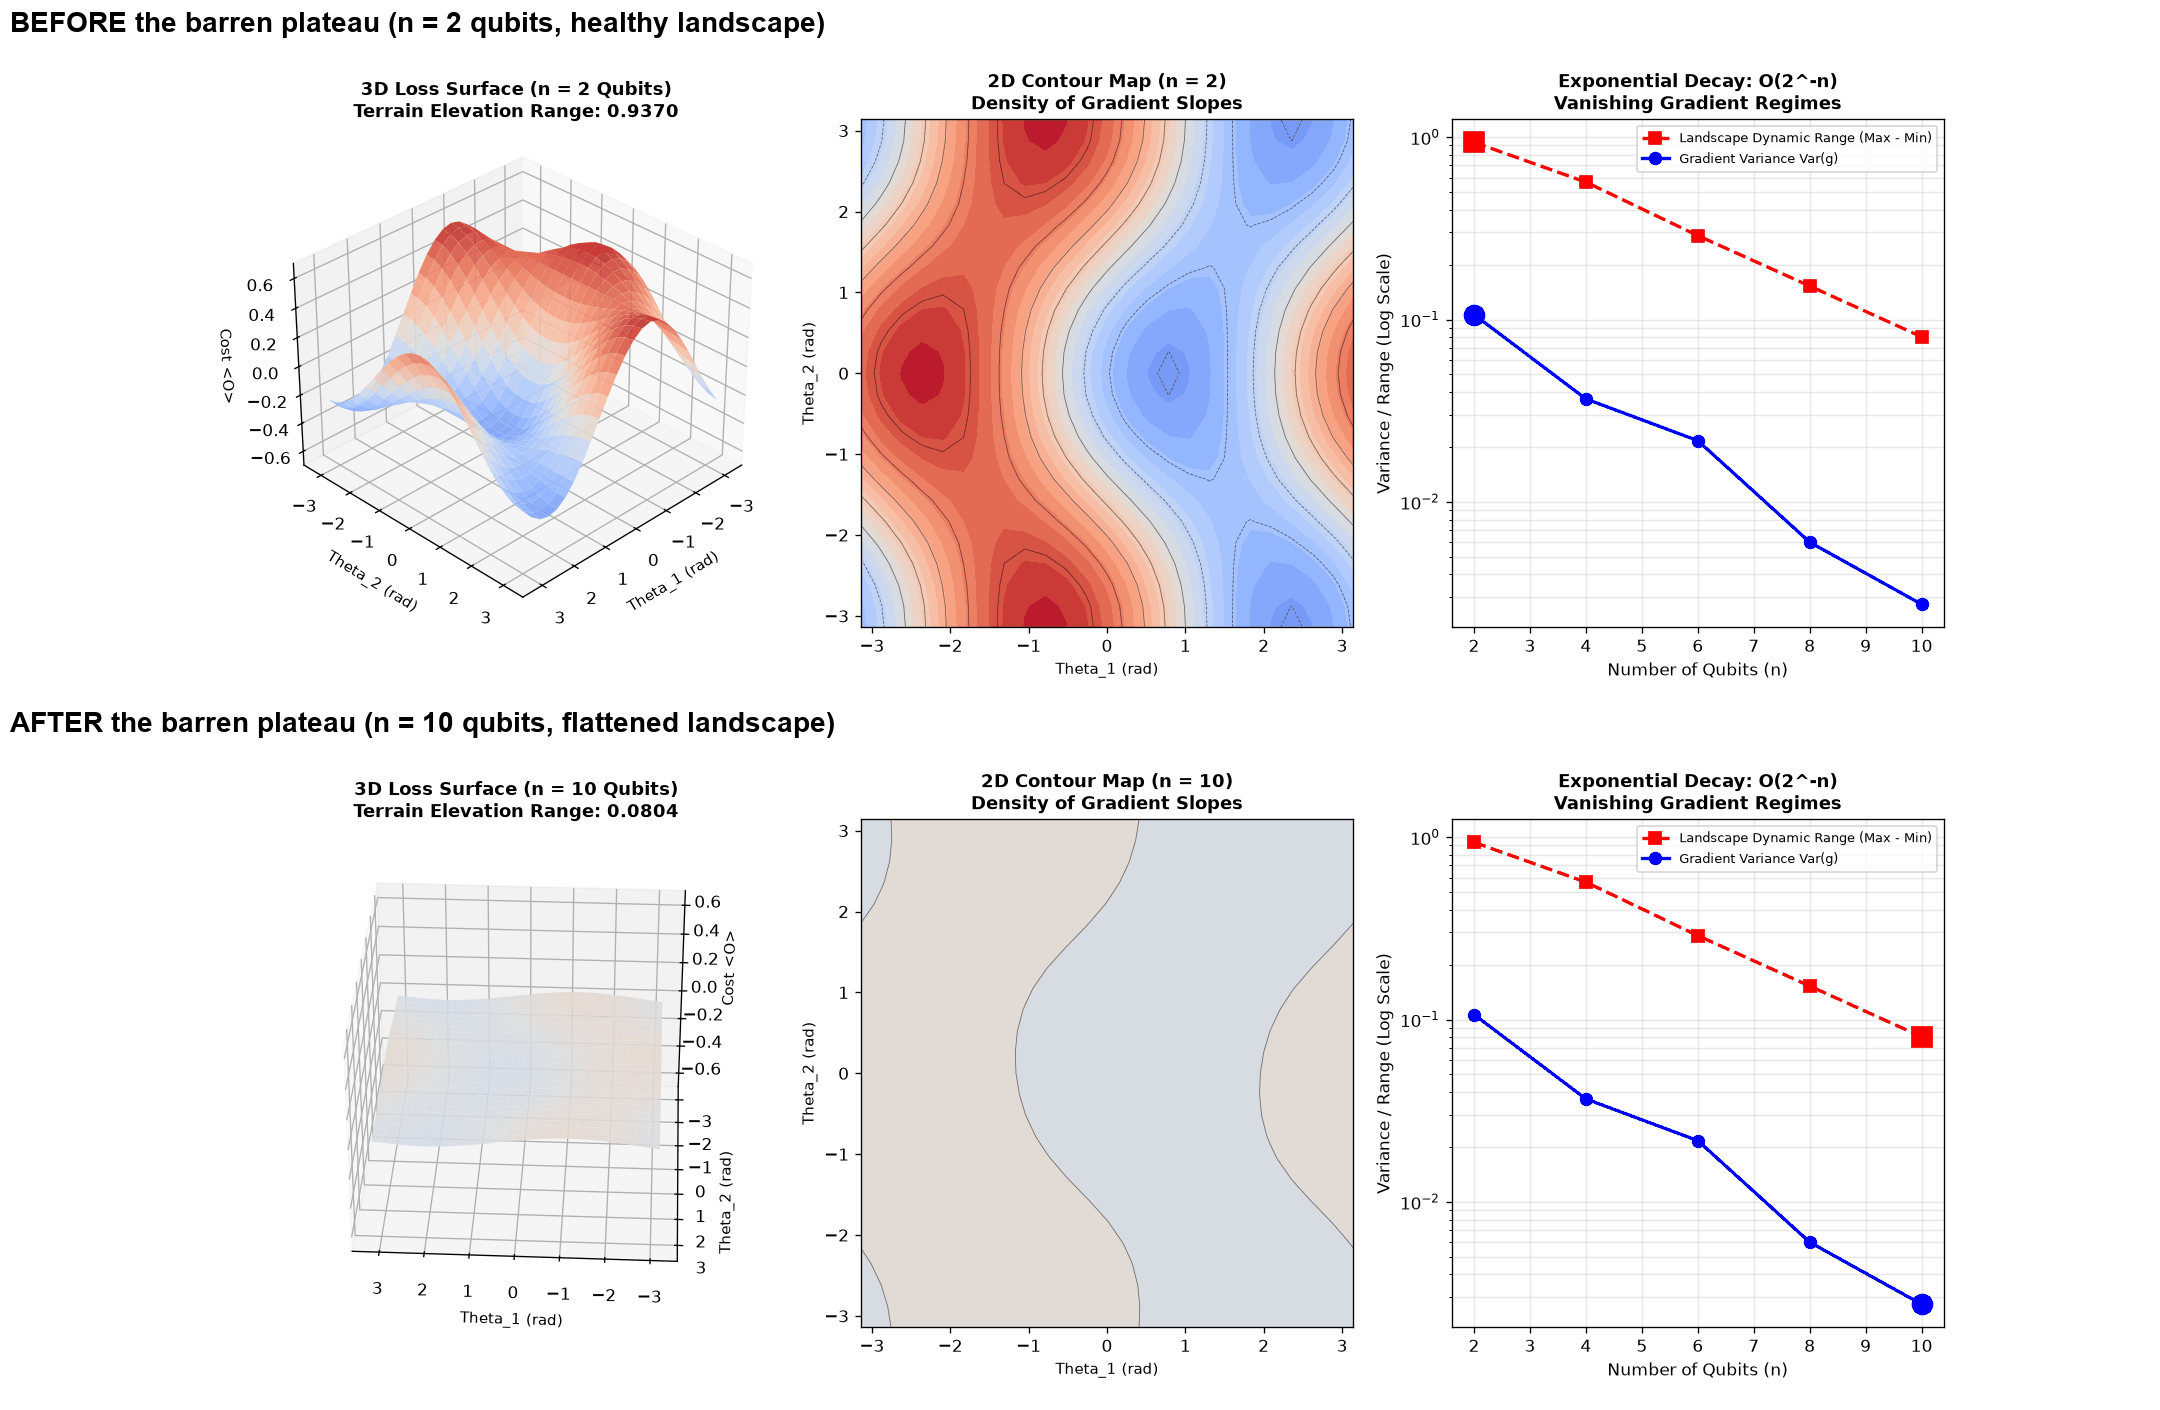
\includegraphics[width=\textwidth]{figure/fig_barren_plateau_theory.png}
\caption{The barren-plateau phenomenon in theory, not an AL-QNN experimental result: the same toy random circuit's cost landscape (left, 3D surface; centre, gradient-slope contour) before the plateau at $n=2$ qubits (top, terrain elevation range 0.937) versus after it at $n=10$ (bottom, range 0.080) -- an $\approx$12$\times$ flattening driven purely by qubit count. The right panel, common to both rows, plots the full $O(2^{-n})$ gradient-variance decay from $n=2$ to $10$, with the marker size highlighting each row's qubit count. This illustrates \citet{mcclean2018barren}'s general result and is independent of the project's own $n\le8$ evaluation scope (Section~1.6, Section~6.1).}
\label{fig:bp_theory}
\end{figure}

\subsection{Causes of Barren Plateaus}
The literature identifies several, partially overlapping, mechanisms that produce barren plateaus, and it is worth distinguishing them because they call for different mitigations.

\subsubsection{Expressivity-Induced Plateaus}
The mechanism formalized by \citet{mcclean2018barren} arises when the ansatz is expressive enough to approximate a 2-design, so that the parameter landscape looks locally random almost everywhere and the gradient variance collapses exponentially with qubit count regardless of what is being optimized. \citet{du2020expressive} formalize this expressivity itself via the circuit's covering number, giving a quantitative basis for the same expressivity-trainability trade-off that motivates treating depth -- not just qubit count -- as a lever on how expressive, and therefore how plateau-prone, the ansatz becomes.

\subsubsection{Cost-Function-Induced Plateaus}
The mechanism refined by \citet{cerezo2021cost} arises separately from how the cost is measured: a global cost that reads out correlations across the whole register concentrates exponentially in the qubit count even for shallow circuits, whereas a local cost that reads out a small, fixed-size subset of qubits only concentrates once the circuit is deep enough for that subset to become entangled with the rest of the system -- which is the origin of the depth-dependent slope measured empirically in Section~6.1.

\subsubsection{Noise-Induced Plateaus and Scope of This Project}
A third, noise-induced mechanism, documented elsewhere in the literature, arises on real hardware from decoherence and gate errors compounding with circuit depth; because this project runs on a noiseless statevector simulator (Section~1.6), noise-induced plateaus are explicitly out of scope, and every plateau observed and mitigated in this report is of the expressivity- or cost-induced kind.

\subsubsection{Relevance to Scheduler Design}
This distinction matters directly for the scheduler design: because the local-cost, depth-dependent plateau is the one this project targets, the reward system (Section~4.7.3) and the recommendation to prefer a local cost (Section~6.4) both follow from \citet{cerezo2021cost}'s result specifically, not from barren-plateau theory in general.

\subsection{Static and Heuristic Mitigation Strategies}
Existing mitigation strategies for barren plateaus fall into three broad categories, each of which informs one part of the baseline comparison in Section~6.

\subsubsection{Structured Initialization}
\citet{grant2019initialization} show that initializing parameters so that the circuit starts close to the identity -- rather than at a uniformly random point -- avoids the plateau at the start of training even for expressive ansätze, because the initial landscape is not yet random. This is a one-time, static intervention: it changes where training starts, not how the architecture evolves during training, which is the gap this project addresses.

\subsubsection{Layerwise Learning}
Related grow-then-freeze heuristics train a circuit one layer at a time, freezing already-trained layers before adding the next. This is conceptually the closest prior approach to AL-QNN's depth scheduling, since both grow the circuit progressively; the difference is that layerwise learning grows on a fixed, pre-determined schedule, while AL-QNN's agent decides whether and when to grow based on live telemetry, and can also prune or freeze growth entirely.

\subsubsection{Adaptive Operator Construction (ADAPT-VQE)}
\citet{grimsley2019adaptive} (ADAPT-VQE) grow an ansatz operator-by-operator, greedily selecting at each step the operator with the largest gradient. This is adaptive in the sense that the final circuit structure is not fixed in advance, but the selection rule itself is a fixed, hand-designed greedy heuristic -- exactly the kind of static policy that AL-QNN's greedy baseline (\Cref{tab:ai4i,tab:heart,tab:sim8g}) formalizes and directly compares against a learned alternative.

\subsection{Reinforcement Learning in Scientific and Quantum Applications}

\subsubsection{RL for Scientific Control Problems}
Reinforcement learning has been applied to a growing range of scientific control problems where the environment is expensive to evaluate and the optimal policy is not known in closed form -- from robotic control to, more recently, quantum circuit design and pulse-level control. A recurring theme in this literature is that the environment's cost of evaluation, not the learning algorithm, is usually the binding constraint: a physical or high-fidelity simulated environment can be too slow to supply the millions of interactions that modern deep RL methods need. This is exactly the constraint that shapes AL-QNN's two-simulator design (Section~4.7.1) -- training against a fast, calibrated surrogate and only deploying the learned policy against the expensive, physically faithful PennyLane backend is the same train-cheap-deploy-faithful pattern behind domain randomization and sim-to-real transfer in robotics \citep{tobin2017domain}, applied here to make training tractable without abandoning a faithful evaluation step.

\subsubsection{Design Philosophy: Off-the-Shelf Algorithms, Domain-Specific MDP}
The two algorithms used in this project, PPO \citep{schulman2017proximal} and DQN \citep{mnih2015human}, are general-purpose deep RL methods with no quantum-specific modification, which is a deliberate design choice: the project's contribution is in how the MDP is constructed around the circuit (Section~4.7), not in a novel RL algorithm. The two were chosen because they represent complementary points in the design space, and neither is assumed a priori to be the better fit for a quantum-telemetry MDP. PPO is on-policy and update-conservative (its clipped objective bounds how far a single update can move the policy), which tends to make training stable but requires fresh interaction data at every update. DQN is off-policy and reuses past interactions through a replay buffer, which can be more sample-efficient but is also more prone to instability when combined with function approximation over a continuous-valued telemetry state. Running both against the identical state, action space, and reward lets Section~6 attribute any performance gap to this stability/sample-efficiency trade-off rather than to an arbitrary choice of algorithm. This mirrors the broader trend in scientific RL applications, where the engineering effort typically goes into designing an informative state and reward from domain telemetry, while the learning algorithm itself is taken off the shelf.

\subsection{Technological Advancements}
Two practical advances make this project feasible.

\subsubsection{Differentiable Quantum Simulation (PennyLane)}
Differentiable quantum-simulation libraries such as PennyLane \citep{bergholm2018pennylane} allow exact statevector gradients via backpropagation, so gradient telemetry can be measured directly. This matters because the standard way to obtain a gradient from a real quantum device -- the parameter-shift rule -- requires evaluating the circuit twice per parameter on hardware, which is affordable for a handful of gradient checks but far too slow to supply the per-epoch gradient-variance telemetry (Section~4.7.2) that the scheduler's state depends on. A statevector simulator sidesteps this entirely: because the full quantum state is available in memory, backpropagation computes every parameter's gradient in a single reverse pass, the same way it would for a classical neural network. This is what makes it computationally realistic to log gradient variance, gradient norm, and the near-zero-gradient ratio at every epoch of every run, rather than only at a few checkpoints.

\subsubsection{Mature Deep Reinforcement Learning Algorithms}
Mature deep reinforcement-learning algorithms -- PPO \citep{schulman2017proximal} and DQN \citep{mnih2015human} -- provide stable policy optimization that can be pointed at the depth-scheduling problem once it is framed as an MDP. Both ship in well-tested open-source implementations with established default hyperparameters, which removes algorithm-level tuning as a variable and lets the experimental effort concentrate on the parts of the system that are specific to this project: the sixteen-dimensional telemetry state, the five-action mutation interface, and the reward weights of \Cref{tab:reward}.

\subsection{Related Work and Research Gaps}

\subsubsection{Comparison of Existing Systems}
\begin{table}[htbp]
\centering
\caption{Comparison of depth-control approaches.}
\label{tab:comparison}
\begin{tabular}{|p{3cm}|p{3.5cm}|p{2.7cm}|p{2.8cm}|}
\hline
\textbf{Approach} & \textbf{Depth control} & \textbf{Uses live telemetry?} & \textbf{Learned?} \\
\hline
Fixed-depth HEA & Manual, fixed & No & No \\
Layerwise learning & Grow-then-freeze, heuristic & Partial & No \\
ADAPT-VQE & Operator growth by gradient & Yes (gradient) & No (greedy) \\
AL-QNN (this work) & Online add/prune of layers & Yes (16-dim telemetry) & Yes (PPO/DQN) \\
\hline
\end{tabular}
\end{table}

\subsubsection{Gaps in the Literature and Justification for the Project}
Existing mitigation strategies are largely static or greedy: they either fix the depth, grow it by a fixed schedule, or add operators one at a time by immediate gradient magnitude. None of them frame depth control as a sequential decision problem in which an agent learns a policy over rich circuit telemetry, and none provide an honest, multi-regime characterization of when such adaptation actually helps versus when a simple rule suffices. This is the gap AL-QNN addresses.

Concretely, each strategy reviewed in Section~3.4 leaves a specific gap that motivates one part of AL-QNN's design. Structured initialization \citep{grant2019initialization} intervenes only once, before training starts, and has nothing to say about how the architecture should evolve once training is underway -- AL-QNN instead makes depth a variable the agent can revisit at every epoch. Layerwise learning grows on a schedule fixed in advance, independent of whether the circuit's gradients are actually healthy at the moment of growth -- AL-QNN conditions every growth decision on the live sixteen-dimensional telemetry state, so a layer is added only when the observed evidence supports it. ADAPT-VQE \citep{grimsley2019adaptive} does use live gradient information, but its selection rule is a fixed, hand-designed greedy heuristic (always add the operator with the largest instantaneous gradient); AL-QNN instead learns the mapping from telemetry to action end-to-end via PPO and DQN, allowing the policy to weigh gradient health against loss trajectory and resource cost jointly, rather than by a single hard-coded criterion. \Cref{tab:comparison} summarizes this progression from manual, to scheduled, to greedy-adaptive, to learned-adaptive depth control.

None of these three prior strategies, nor the reinforcement-learning applications surveyed in Section~3.5, report results across multiple cost-type regimes with an explicit accounting of where the approach fails. This project's empirical contribution is therefore not only the learned scheduler itself, but the multi-regime evaluation of Section~6, which is designed specifically to expose the boundary between the regime where adaptive scheduling helps and the regime where it does not -- a boundary that the reviewed literature does not characterize because none of the reviewed methods are evaluated against a matched static baseline across more than one regime.

\section{Methodology}
This project applies reinforcement learning to control the architecture of a quantum circuit during training. The methodology below covers the machine-learning side (data, model, evaluation protocol) and the reinforcement-learning side (environment, agent, reward) of the system.

\begin{figure}[htbp]
\centering
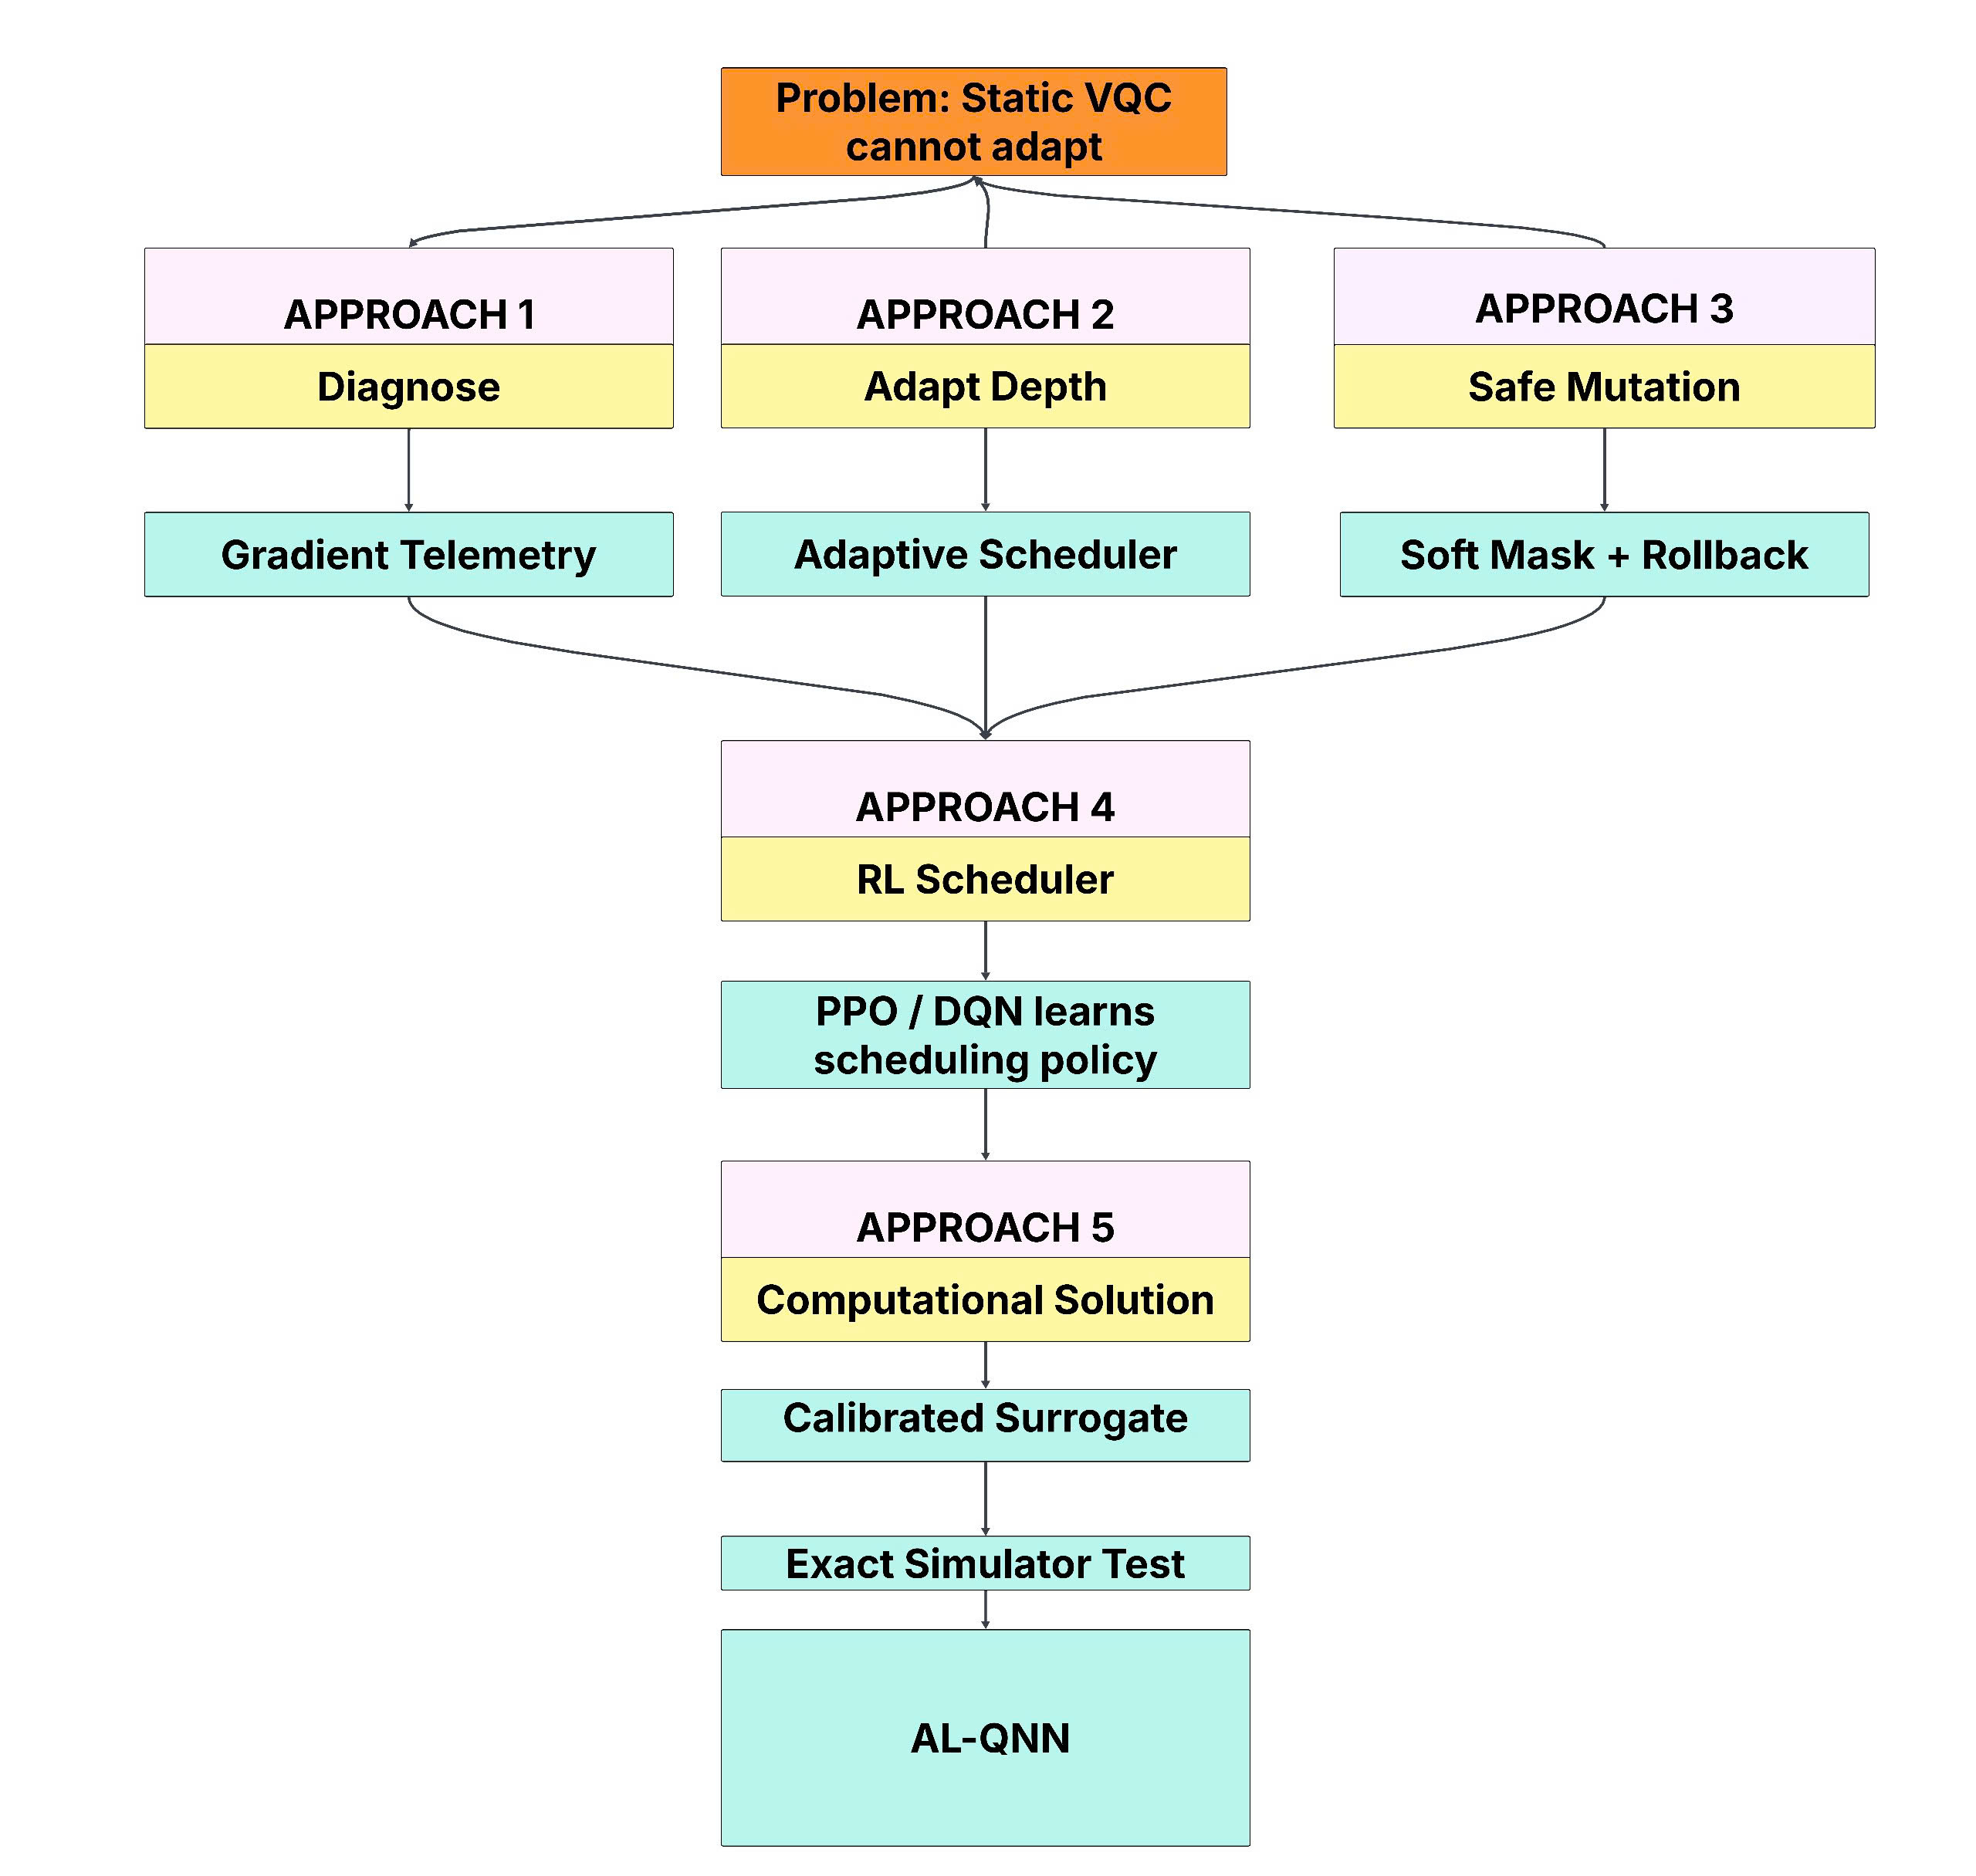
\includegraphics[width=0.7\textwidth]{figure/fig_solution_approach.jpg}
\caption{From problem to solution. A static VQC cannot adapt (top); Approaches 1--3 diagnose circuit health via gradient telemetry (Section~4.4.1), adapt depth via a scheduler (Section~4.4.2), and apply changes through safe, reversible mutation (Section~4.4.3); Approach~4 learns this diagnose-adapt-mutate policy end-to-end with PPO/DQN (Section~4.4.4); and Approach~5 makes that learning computationally tractable by training on a calibrated surrogate before evaluating on an exact PennyLane simulator (Section~4.4.5) -- together defining AL-QNN.}
\label{fig:solution_approach}
\end{figure}

\subsection{Research Questions and Objectives}

\subsubsection{Research Questions}
The project addresses three research questions. RQ1: can a variational quantum classifier built from a hardware-efficient ansatz reach competitive accuracy on real tabular datasets at NISQ-scale qubit counts? RQ2: to what extent does the barren plateau limit trainability at these scales, and how does that limit depend on the cost function and the circuit depth? RQ3: does scheduling the circuit depth (rather than fixing it) improve or at least match a well-tuned fixed-depth model?

\subsubsection{Project Objectives}
The objective is to build the classifier, measure the barren plateau empirically, and evaluate performance under a consistent, leakage-free protocol.

\subsection{Data}

\subsubsection{Dataset Collection Overview}
The project data package contains several binary-classification tabular datasets spanning healthcare, finance, and industrial maintenance. This section covers only the datasets for which a scheduler-comparison run was actually logged and reported in Section~6 (\Cref{tab:datasets}); the loader also supports a few additional datasets (a high-dimensional image case and a small clean benchmark) that were used only for earlier smoke-testing and preprocessing checks and never carried through to a logged comparison run, and are therefore left out of this report entirely rather than described without matching results. Dataset facts below (native instance and feature counts, provenance) are attributed to the original dataset authors or their UCI Machine Learning Repository records; project-specific sample counts, feature selection, class balancing, and encoding steps are attributed to the AL-QNN project's data-preparation scripts and loader (\texttt{data/prepare\_*.py}, \texttt{scripts/dataset.py}).

\subsubsection{Common Data Preparation Pipeline}
Preprocessing is deterministic and strictly fit on the training split to prevent leakage. The project loader converts each dataset to a binary target, then applies a fixed-seed stratified split into train, validation, and test; a Z-score standardization is fitted on the training split and applied to all splits; the feature count is then reconciled with the requested qubit count in one of three ways -- principal-component analysis (PCA), fitted on the training data, when the native feature count exceeds the qubit count; a direct one-to-one mapping when the two are equal; or zero-padding with constant, uninformative columns when the native feature count is smaller than the requested qubit count -- and finally every feature is rescaled to the angle-encoding range [0, π]. None of the five datasets reported in Section~6 currently needs the zero-padding case at their evaluated qubit count; it remains a supported loader behaviour for a dataset whose native feature count is smaller than the requested qubit count, kept honest here rather than described as if exercised. Missing values (for example in the Heart dataset) are removed before splitting. Several datasets are also balanced to an even class ratio by undersampling the majority class, which makes scheduler comparisons less dependent on class imbalance but means the processed files should not be read as representative of the original class distributions; AI4I is the one exception to undersampling (Section~4.2, AI4I 2020 Predictive Maintenance). This end-to-end flow runs from the raw per-dataset CSV to the angle-encoded input consumed by the hardware-efficient ansatz of Section~4.4.2, and this final $[0,\pi]$ encoding step is shared by all five datasets below, not just AI4I.

\begin{figure}[htbp]
\centering
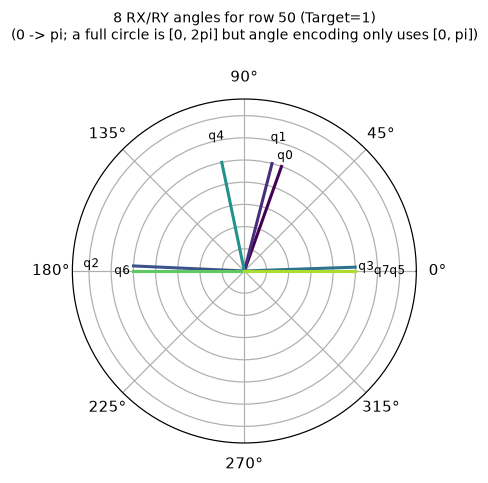
\includegraphics[width=0.55\textwidth]{figure/output.png}
\caption{A worked example of the final angle-encoding step every dataset in \Cref{tab:datasets} goes through: the eight $R_X$/$R_Y$ rotation angles produced by encoding a single training row (an AI4I failure case, shown here as a concrete instance), plotted on $[0,\pi]$ of a polar axis to show that no encoded angle exceeds the half-circle the ansatz actually uses.}
\label{fig:angle_example}
\end{figure}

\FloatBarrier
\subsubsection{Pima Indians Diabetes}
The Pima Indians Diabetes dataset records 768 observations of women of Pima Indian heritage, at least 21 years old, with eight predictive variables covering pregnancies, glucose, blood pressure, skin thickness, insulin, BMI, diabetes pedigree function, and age; the original class split is imbalanced at 268 positive versus 500 negative cases \citep{smith1988pima}. The project's preparation script balances the classes to 536 observations (268 per class) and retains all eight original predictive variables without PCA, since eight features already matches the eight-qubit target register. This gives a direct 8-feature-to-8-qubit mapping, making Pima useful for isolating the effect of circuit depth and adaptive scheduling from any dimensionality-reduction confound; it contributes one of the supplementary single-seed deployments reported in \Cref{tab:pima} (Section~6.1).

\subsubsection{Heart Disease -- Cleveland}
The UCI Cleveland Heart Disease record describes 303 instances and 13 predictive attributes -- age, sex, chest-pain type, resting blood pressure, cholesterol, fasting blood sugar, resting ECG, maximum heart rate, exercise-induced angina, ST depression, slope, number of major vessels, and thalassemia -- with an original five-level target that is conventionally binarized to absence (0) versus presence (1--4) of disease \citep{detrano1989heart}. The project's preparation script follows this binary convention, removes rows with missing values, balances the resulting classes, and applies \texttt{SelectKBest} with an ANOVA F-test to reduce 13 features to the 8 most informative ones, yielding 274 processed observations (137 per class). This dataset is used both for the AI4I-style barren-plateau characterization and, later, for the real PennyLane deployment reported in \Cref{tab:heart}.

\subsubsection{Parkinson's -- Oxford Parkinson's Disease Detection Dataset}
The UCI Parkinsons record uses biomedical voice measurements -- fundamental-frequency measures, jitter, shimmer, noise-to-harmonics ratios, and nonlinear dynamical measures -- drawn from 195 voice recordings of 31 people (23 with Parkinson's disease), reported as 197 instances over 22 features \citep{little2007parkinsons}. The project's preparation script selects 8 features from the original 22 with \texttt{SelectKBest} and balances the classes to a 96-observation set (48 per class). Its small sample size makes this dataset useful for probing scheduler stability under sensitivity to the train/validation split and random seed, and it contributes one of the supplementary single-seed deployments reported in \Cref{tab:parkinsons} (Section~6.1).

\subsubsection{Statlog German Credit}
The Statlog German Credit dataset contains 1,000 instances and 20 categorical and integer attributes describing applicants as good or bad credit risks \citep{hofmann1994german}. The project's preparation script converts categorical values to numerical category codes, binarizes the credit-risk label, balances the classes to 600 observations (300 per class), and selects 8 features from the original 20 with \texttt{SelectKBest}, producing a file directly compatible with an eight-qubit input representation. A Logistic Regression cross-validation sanity check on the processed file reports approximately 0.725 accuracy, which the project treats as a moderate classification difficulty suitable for scheduler comparison; German Credit is accordingly used for one of the supplementary single-seed scheduler-comparison deployments reported alongside AI4I and Heart Disease in \Cref{tab:german} (Section~6.1).

\subsubsection{AI4I 2020 Predictive Maintenance}
The AI4I 2020 Predictive Maintenance dataset is a synthetic industrial dataset of 10,000 observations, multivariate and time-series in nature, whose binary machine-failure label is set to 1 when at least one of several defined failure modes occurs \citep{matzka2020ai4i}. The project representation combines five numerical process/sensor variables with the three one-hot-encoded categories of the machine \texttt{Type} field to produce a fixed 8-column engineered input. The raw label is strongly imbalanced (9,661 non-failure vs 339 failure, $\approx$3.4\% positive); the loader preserves this natural ratio when reading the data, stratified-subsampling only if a smaller \texttt{max\_samples} budget is requested, rather than discarding real majority-class rows just to force balance. Class balance is instead restored by SMOTE \citep{chawla2002smote}, applied only to the training split, only after the train/validation/test split and after the one-to-one feature mapping and $[0,\pi]$ angle-encoding scaling described below -- so synthetic points are interpolated in the same already-encoded space the ansatz consumes, and the validation and test splits are left at the true $\approx$3.4\% ratio for an honest evaluation. This fixed 8-column representation maps one-to-one onto the project's 8-qubit scope (Section~1.6), the same direct mapping as Pima, so the primary result table (\Cref{tab:ai4i}, three seeds, $n=8$) runs on 8 real, independently informative features with no dimensionality reduction or padding involved. AI4I is nonetheless the project's primary dataset, chosen in part because it tests whether a scheduler remains effective under an application domain with severe native class imbalance and multiple physical operating variables, rather than only on small, already-clean academic benchmarks.

\begin{figure}[htbp]
\centering
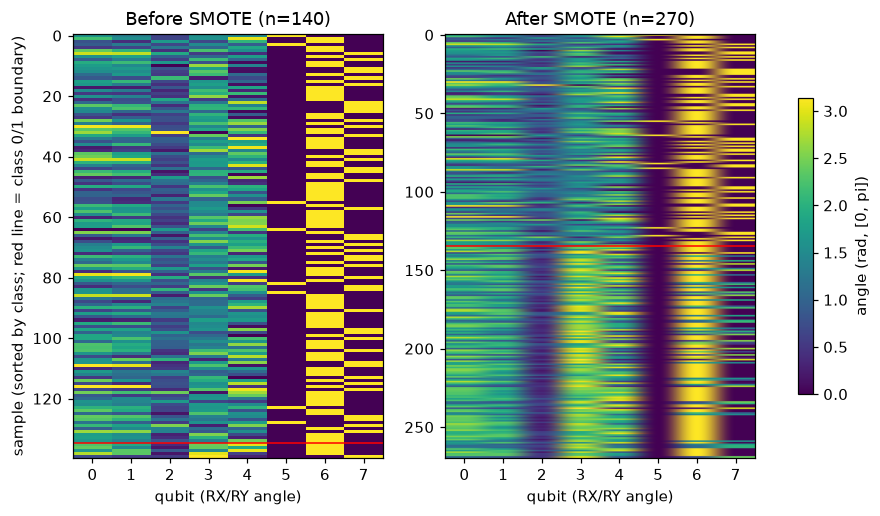
\includegraphics[width=0.95\textwidth]{figure/before_vs_after_SMOTE.png}
\caption{A representative training-split subset's angle-encoded features (one column per qubit) before and after SMOTE, samples sorted by class with the class-0/1 boundary marked in red. Every value stays inside $[0,\pi]$ because SMOTE interpolates directly in the already fit-and-scaled encoding space (Section~4.2), not in raw feature space.}
\label{fig:smote_angles}
\end{figure}

\begin{figure}[htbp]
\centering
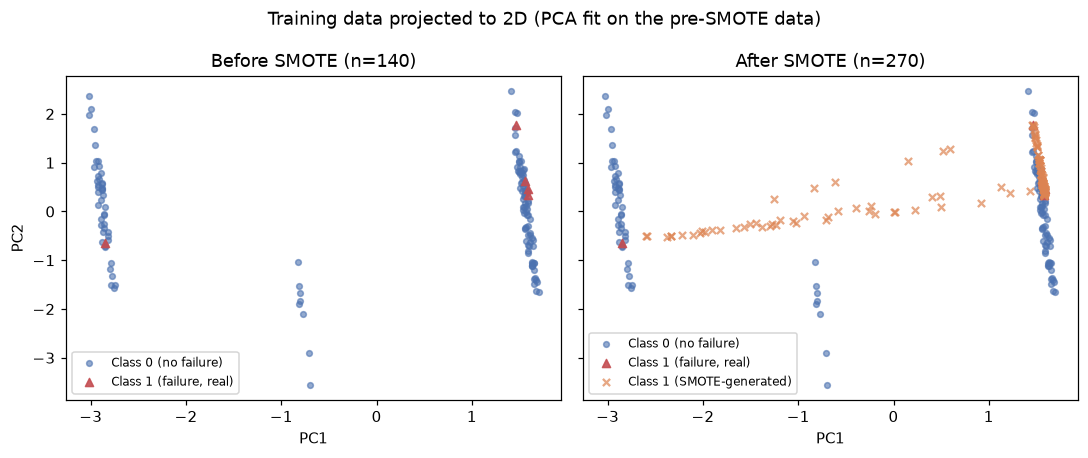
\includegraphics[width=0.85\textwidth]{figure/smott.png}
\caption{The same training-split subset projected onto its first two principal components (PCA fit on the pre-SMOTE data, for visualization only -- AI4I itself uses no PCA at $n=8$, per \Cref{tab:datasets}). SMOTE-generated failure samples (orange) interpolate between the real failure samples (red) rather than forming an unrelated cluster, which is the qualitative check this figure exists to make.}
\label{fig:smote_pca}
\end{figure}


\begin{table}[htbp]
\centering
\caption{Datasets used, their native feature count, and the qubit-count/feature-reduction mapping applied.}
\label{tab:datasets}
\begin{tabular}{|p{3.4cm}|p{2.6cm}|p{2.2cm}|p{4.6cm}|}
\hline
\textbf{Dataset} & \textbf{Native features} & \textbf{Qubits used} & \textbf{Reduction applied} \\
\hline
AI4I 2020 (predictive maintenance) & 8 (fixed: 5 numeric + 3 one-hot) & 8 & None -- one-to-one mapping \\
Heart Disease (Cleveland) & 13 & 8 & Univariate feature selection, 13 to 8 \\
Parkinson's & 22 & 8 & Univariate feature selection, 22 to 8 \\
Pima Diabetes & 8 & 8 & None -- one-to-one mapping \\
German Credit (Statlog) & 20 & 8 & Univariate feature selection, 20 to 8 \\
\hline
\end{tabular}
\end{table}

\subsubsection{Dataset Suitability and Usage Across Experiments}
AI4I 2020 predictive maintenance is the primary dataset (\Cref{tab:ai4i}, three seeds) and Heart Disease is the dataset behind the primary real PennyLane deployment (\Cref{tab:heart}); together these anchor the core evaluation design of Section~6.1--6.2. German Credit, Parkinson's, and Pima each contribute one additional single-seed PennyLane deployment, reported as supplementary evidence in \Cref{tab:german,tab:parkinsons,tab:pima} (Section~6.1) rather than as part of the core design itself. Taken together, the five datasets kept in this report are deliberately heterogeneous: Pima and Heart give, respectively, a direct feature-to-qubit case and a feature-selection case on real medical data; Parkinson's stresses scheduler stability on a small sample; and German Credit and AI4I supply moderate-difficulty financial and severely-imbalanced industrial benchmarks. A scheduler that only performs well on one simple dataset would not be expected to generalize across this range of sample size, class balance, and preprocessing requirements, which is why Section~6 draws its regimes and supplementary checks from more than one of these sources rather than reporting a single dataset's results.

\subsection{Feature Selection and Engineering}

\subsubsection{Feature-to-Qubit Mapping}
The number of input features is matched to the qubit count. Where a dataset already has exactly as many informative features as qubits -- Pima and AI4I with eight features each for eight qubits -- the mapping is one-to-one and no dimensionality reduction is applied, preserving all information. Where there are more features than qubits, the dimension is reduced by univariate feature selection via \texttt{SelectKBest} (Heart, 13 $\rightarrow$ 8; Parkinson's, 22 $\rightarrow$ 8; German Credit, 20 $\rightarrow$ 8); none of the five datasets reported in Section~6 currently needs PCA or zero-padding at their evaluated qubit count, though the loader supports both (Section~4.2, Common Data Preparation Pipeline) and PCA remains the intended route for a higher-dimensional or less individually-interpretable feature set, such as the image and small-benchmark cases mentioned in Section~4.2 that were used only for smoke-testing. Each selected feature is then engineered into a rotation angle in [0, π] by angle encoding.

\subsubsection{Choice of Reduction Strategy}
Univariate selection is used for every dataset in this report that needs reduction at all -- Heart, Parkinson's, and German Credit -- because their raw features are already individually interpretable clinical, demographic, or financial measurements, so discarding the least informative ones preserves the meaning of the remaining features and keeps the angle-encoding mapping interpretable feature-by-feature. PCA was used in an earlier, wider-qubit-range version of this project for AI4I's fixed, sensor-derived feature set; at the project's current 8-qubit scope AI4I's 8 native features map one-to-one onto 8 qubits instead (Section~4.2, AI4I 2020 Predictive Maintenance), so no dataset currently reported in Section~6 exercises the PCA path, though it remains available for a higher-dimensional or less individually-interpretable feature set should one be added. Both reduction strategies converge on the same downstream representation -- exactly \$n\$ real-valued features per sample, rescaled to [0, π] -- so that the ansatz and the RL environment never need to know which reduction strategy produced their input: Z-score standardization reshapes each raw feature's distribution, PCA or \texttt{SelectKBest} reduce $n$ raw features down to $k$ qubit features, and the resulting $k$-dimensional vector is rescaled into $[0,\pi]$ and loaded as a per-qubit $R_Y(\theta_i)$ rotation.

\subsection{Approach Overview: Diagnose, Adapt, Mutate Safely}
\quad Five coupled sub-problems must be solved for a scheduler to safely and practically control circuit depth: diagnosing the circuit's true state (Approach~1), deciding what structural change that state calls for (Approach~2), applying any change without risking the run (Approach~3), learning the diagnose-to-action mapping end-to-end rather than hand-coding it (Approach~4), and making that learning loop computationally tractable in the first place (Approach~5). \Cref{fig:solution_approach} at the start of this chapter traces exactly this chain from problem to the finished AL-QNN system; the five subsections below introduce each briefly, with full technical detail in Section~4.4.2 (circuit model) and Section~4.7 (environment, agent, reward). \Cref{tab:approach_io} summarizes what each approach consumes and produces, so the chain from raw telemetry to a deployed policy can be followed at a glance before the detail.

\begin{table}[htbp]
\centering
\caption{Input and output of each approach.}
\label{tab:approach_io}
\begin{tabular}{|p{2.6cm}|p{5.3cm}|p{5.3cm}|}
\hline
\textbf{Approach} & \textbf{Input} & \textbf{Output} \\
\hline
1: Diagnosis & Five raw runtime signals per epoch; offline Stage~1C risk table & One of five diagnosis labels -- logged (Appendix~B), fed into the state (\Cref{tab:state}), gates $w_1$ (\Cref{tab:reward}) \\
2: Scheduling & Diagnosis label (Approach~1); current depth and depth cap & Masked space of legal actions from \Cref{tab:actions} \\
3: Safe Mutation & Agent-selected structural action (Approach~4); checkpointed parameters & Committed circuit (gates removed) or rolled-back circuit (checkpoint restored) \\
4: RL Scheduler & Sixteen-dimensional telemetry state (\Cref{tab:state}) & One selected action from \Cref{tab:actions}, trained on the reward of \Cref{tab:reward} \\
5: Computational Solution & Stage~1 barren-plateau measurements & Trained policy, deployed and evaluated on PennyLane (Section~6) \\
\hline
\end{tabular}
\end{table}

\subsubsection{Approach 1: Multi-Dimensional Gradient Telemetry and Diagnosis}
A naive rule -- flag a barren plateau whenever the gradient norm drops below a threshold -- cannot tell a true plateau apart from ordinary behaviour that looks the same: convergence, a local minimum, one dead layer amid otherwise healthy ones, or plain shot noise. Approach~1 instead diagnoses the circuit every epoch from five raw runtime signals $\mathbf{s} \in \mathbb{R}^5$, mapped to continuous risk probabilities by a sigmoid,
\begin{equation}
p_k = \sigma(s_k) = \frac{1}{1+e^{-s_k}}, \qquad k = 1,\dots,5,
\end{equation}
and checked against the offline risk table calibrated in Stage~1C from the Stage~1 barren-plateau measurements (Section~4.7.1). A fixed priority order resolves these probabilities into exactly one label: \textbf{solved/converged} (loss at target -- locks out further mutation), \textbf{local minimum} (loss flat, gradient still non-trivial -- keep optimizing), \textbf{dead layer} (one layer's gradient collapsed, rest healthy -- mask that layer only), \textbf{ambiguous} (inconclusive -- watch, don't act), or \textbf{true barren plateau} (every layer collapsed under high structural risk -- lock depth growth). The label is logged every epoch (\texttt{is\_solved}, \texttt{is\_converged}, \texttt{is\_local\_min}, \texttt{is\_dead\_layer}, \texttt{is\_ambiguous}, \texttt{is\_true\_bp}, Appendix~B), feeds the agent's sixteen-dimensional state (\Cref{tab:state}), and gates the reward directly: once solved, the gradient-variance weight ($w_1$ in \Cref{tab:reward}) is forced toward zero so the agent cannot keep collecting reward by disturbing a converged model.

\subsubsection{Approach 2: Adaptive Circuit Scheduling}
Once the circuit's state is known, the question becomes what to do about it. Each layer $\ell$ of the ansatz follows the hardware-efficient ansatz pattern of \citet{kandala2017hardware}: a single-qubit rotation block on every qubit followed by a fixed entangling layer. Concretely, each layer applies, to every qubit $i \in \{1, \dots, n\}$, the single-qubit Euler decomposition
\begin{equation}
U_i^{(\ell)}(\theta) = R_Z(\theta_{i,3}^{(\ell)})\, R_Y(\theta_{i,2}^{(\ell)})\, R_Z(\theta_{i,1}^{(\ell)})
\end{equation}
followed by a fixed nearest-neighbour entangling layer $\mathrm{CNOT}_{i,i+1}$ applied for $i = 1, \dots, n-1$. A depth-$d$ circuit is then the ordered product
\begin{equation}
U(\theta) = \prod_{\ell=1}^{d} \left( \prod_{i=1}^{n-1} \mathrm{CNOT}_{i,i+1} \right) \left( \bigotimes_{i=1}^{n} U_i^{(\ell)}(\theta) \right)
\end{equation}
acting on the angle-encoded input state, with the classification output read from a measurement of the final state. The global cost used in Section~1.4's problem statement is a function of the full $n$-qubit measurement outcome, whereas the local cost this project targets restricts each cost term to a small subset of qubits (following the construction of \citet{cerezo2021cost}); this is what weakens the exponential qubit-count scaling of the gradient variance into the depth-dependent behaviour exploited by the scheduler throughout Section~6.

This ansatz was chosen because it is expressive, respects device connectivity, and keeps circuits shallow -- the properties required on NISQ hardware. At 8 qubits each layer contributes 24 trainable parameters (8 qubits $\times$ 3 rotations); the circuit therefore holds 24$\times$depth parameters, e.g. 48 at depth 2 and 120 at depth 5. The depth is bounded by a cap (typically 6-16 depending on the qubit count).

A static hardware-efficient ansatz fixes $D(t) = D_{\text{fixed}}$ for every epoch $t$; Approach~2 instead makes depth $D(t)$ a variable the agent controls through the five discrete actions of \Cref{tab:actions} -- adding a layer when expressivity is needed and gradients are healthy, holding while the optimizer converges, stopping growth once Approach~1 flags solved or true-barren-plateau risk, and proposing to prune a layer or reduce entanglement when only part of the circuit is diagnosed as harmful. An action mask, rebuilt each epoch from the current depth, the depth cap, and the diagnosis state, removes illegal or unsafe actions before the agent ever selects among them (Section~4.7.2), so the learned policy always stays inside hardware-consistent bounds.

\subsubsection{Approach 3: Safe Mutation via Soft-Masking and Registry Rollback}
A structural change proposed under Approach~2 might hurt training, so no mutation is ever applied irreversibly. A layer proposed for pruning or entanglement reduction is first soft-masked rather than deleted: a coefficient $S(t)$ scales its contribution and decays over a short window of $T$ epochs (5 by default) on a cosine schedule \citep{loshchilov2017sgdr},
\begin{equation}
S(t) = \tfrac{1}{2}\bigl[1+\cos(\pi t / T)\bigr], \qquad t = 0,\dots,T,
\end{equation}
chosen because $\mathrm{d}S/\mathrm{d}t = 0$ at both endpoints, so masking introduces no abrupt jump that would desynchronize the Adam optimizer's momentum buffers. The circuit's parameters are checkpointed in a parameter registry before masking begins; at the end of the window the mutation is \textbf{committed} (gates permanently removed) if the worst loss reached during the window stayed within tolerance,
\begin{equation}
\frac{\mathcal{L}_{\text{peak}} - \mathcal{L}_{\text{start}}}{\mathcal{L}_{\text{start}}} \;\le\; \delta \quad (\delta = 0.02 \text{ by default}),
\end{equation}
and \textbf{rolled back} to the exact checkpointed state otherwise -- tracking the peak rather than the final-epoch loss so that mid-window damage cannot be hidden by late recovery. Algorithm~1 (Section~4.7.4) formalizes this loop; it is what lets the scheduler explore structural changes -- something a static ansatz can never do -- without risking permanent damage to a run that was already working.

\subsubsection{Approach 4: RL Scheduler}
Approaches 1--3 define what the agent perceives and what it may do, but not how it decides. Approach~4 learns that mapping end-to-end instead of hand-coding it: the sixteen-dimensional telemetry state (\Cref{tab:state}) is fed to a PPO \citep{schulman2017proximal} or DQN \citep{mnih2015human} agent, which outputs one of the five actions of \Cref{tab:actions} every epoch and is trained to maximize the weighted reward of \Cref{tab:reward}. This favours a general-purpose, off-the-shelf algorithm over a hand-designed heuristic (Section~3.5.2): the project's contribution is the state, action, and reward design around the circuit, not a new RL algorithm. Full agent, state, and reward design is given in Section~4.7.2--4.7.4.

\subsubsection{Approach 5: Computational Solution}
Training Approach~4's agent needs millions of environment interactions, but an exact circuit gradient on real quantum hardware requires the parameter-shift rule -- two circuit evaluations per parameter,
\begin{equation}
g_i = \frac{\mathcal{L}(\theta_i + \tfrac{\pi}{2}) - \mathcal{L}(\theta_i - \tfrac{\pi}{2})}{2},
\end{equation}
per \citet{mitarai2018quantum,schuld2019evaluating} -- far too slow to repeat every epoch of every episode. Approach~5 resolves this with the two-simulator design: PPO/DQN train against a fast classical surrogate calibrated on the Stage~1 measurements, while only the final learned policy is deployed and evaluated on PennyLane's exact statevector backend (Section~4.7.1), which obtains the same gradient by backpropagation in a single reverse pass instead of one parameter-shift evaluation at a time. Every number reported in Section~6 comes from this exact-simulator deployment, never from the surrogate alone.

\subsection{Training Configuration}
Training uses exact statevector gradients (backpropagation) on the PennyLane simulator for 40 deployment epochs. Data are split deterministically by a fixed data-split seed (42) into 70\% train and 30\% validation; the deployment and comparison scripts (\texttt{scripts/04\_train\_rl\_scheduler.py}, \texttt{scripts/05\_compare\_schedulers.py}) do not carve out a separate held-out test split for the results in Section~6, so the accuracy, F1, and ROC AUC numbers reported throughout are computed on the validation split -- the same split the scheduler observes every epoch to make its accept/rollback decisions. This is an honestly-reported limitation rather than a leakage bug: no scaler, PCA, or model parameter is ever fit on the validation data, but because the scheduler's structural decisions are themselves conditioned on validation performance, the reported numbers should be read as in-loop validation metrics rather than metrics from data the pipeline never touched. A separate three-way train/validation/test split exists in the shared data loader (\texttt{test\_frac}) and is used by the standalone prediction-export script (\texttt{export\_predictions.py}) that backs the demonstration interface, but it is not the configuration behind either the three-seed AI4I variance check or the single-seed comparison tables in Section~6. AI4I was additionally validated with three random seeds during development (reported as mean $\pm$ standard deviation) to characterize seed variance; the scheduler-comparison tables presented in Section~6 are single-seed and treated as exploratory.

\subsection{Evaluation Metrics}

\subsubsection{Classification and Trainability Metrics}
Classification quality is measured by accuracy, F1 score, and ROC AUC on the validation split (Section~4.5), which is the only non-training split available in the single-seed comparison runs behind Section~6. Trainability is measured by the spatial gradient variance and the near-zero-gradient ratio, which quantify how close the model is to a barren plateau.

\subsubsection{Resource and Scheduler-Behaviour Metrics}
Resource use is measured by the final circuit depth and the number of entangling gates. The scheduler's behaviour is characterized by the number of committed and rolled-back mutations. Metrics from the three-seed AI4I variance check (Section~6.1) are reported as a mean with standard deviation; the scheduler-comparison tables in Section~6 are single-seed.

\subsection{The Reinforcement-Learning Environment}
\subsubsection{Environment Setup}
An episode corresponds to one full training run of the variational classifier under the agent's depth-scheduling decisions. At the start of an episode the circuit is initialized at a starting depth (typically 2); at each step the agent observes the current telemetry, chooses one action (Section~4.7.2), and the environment executes one epoch of parameter optimization under the resulting architecture before returning the next state and reward (Section~4.7.3). An episode ends after a fixed epoch budget or when the depth cap is reached and no further mutation is possible. The environment is configured by four parameters that are held fixed within a run: the dataset, the qubit count, the cost type (local or global), and the depth bounds (initial depth and maximum depth).

Critically, the same environment interface -- the same state, the same actions, the same reward -- is implemented on top of two interchangeable physics backends, and the choice between them is the central engineering trade-off of the project.

The \textbf{simulate} backend drives the environment with a calibrated classical surrogate -- an application, in this depth-scheduling setting, of the broader result that classical models can faithfully stand in for certain quantum learning models \citep{schreiber2023classical}: closed-form numpy functions for the loss floor and the gradient variance as a function of depth, qubit count, and cost type, fit to the real measurements collected during Stage 1 (barren-plateau characterization) by nonlinear least-squares regression. A step costs microseconds, which is what makes it possible to run the millions of environment steps PPO and DQN need -- training an agent this way takes on the order of thirty minutes. What is lost is physical fidelity: the surrogate reproduces the calibrated trend (loss decreasing with depth up to a point, gradient variance decaying with qubit count, the local-vs-global depth slope), not an exact quantum state or a true autodiff gradient, and it is only as reliable as the regime it was calibrated on -- extrapolating it to an untested qubit count, cost type, or ansatz can silently diverge from the real circuit, which is why the surrogate is explicitly re-calibrated whenever any of those change.

The \textbf{PennyLane} backend \citep{bergholm2018pennylane} drives the environment with the real hardware-efficient circuit: an actual statevector is prepared, and the loss and gradient variance are computed by backpropagation through it, so the physics is exact. This is why every number reported in Section~6 is produced by a PennyLane deployment run, never by the surrogate. The cost is speed, and this is measured rather than assumed: one epoch on a 270-sample training batch at $n=8$ qubits takes 18.3\,s, and epoch time scales linearly with the sample count (\Cref{fig:time_per_ep}), so a single epoch over the full 10,000-row AI4I dataset would cost 679\,s ($\approx$11.3\,min). Carried out over the 600 episodes PPO is trained for (Section~4.7.4), that per-epoch cost compounds to roughly 283 days of wall-clock time for one agent (\Cref{fig:time_to_train}) -- a month's worth of training reached only by episode 64 -- which is why PennyLane is used only for deployment and evaluation (40 epochs), never for the RL training loop itself.

\begin{figure}[htbp]
\centering
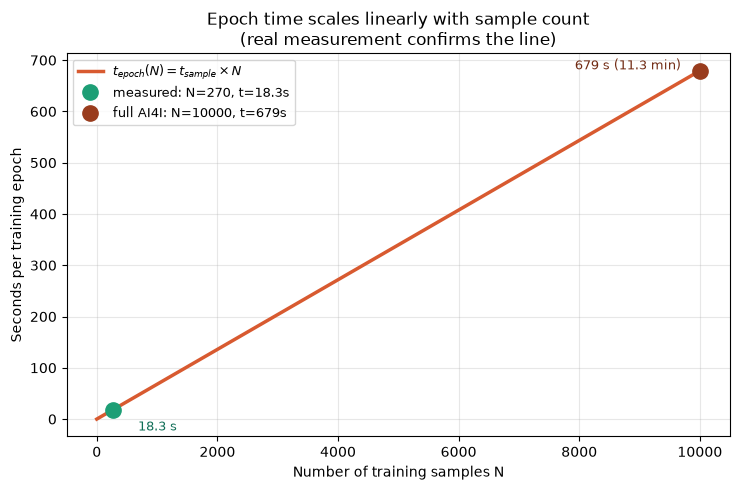
\includegraphics[width=0.75\textwidth]{figure/time_per_ep.png}
\caption{Measured PennyLane epoch time versus training-sample count at $n=8$ qubits (270 samples, 18.3\,s), extrapolated linearly to the full 10,000-row AI4I dataset (679\,s per epoch).}
\label{fig:time_per_ep}
\end{figure}

\begin{figure}[htbp]
\centering
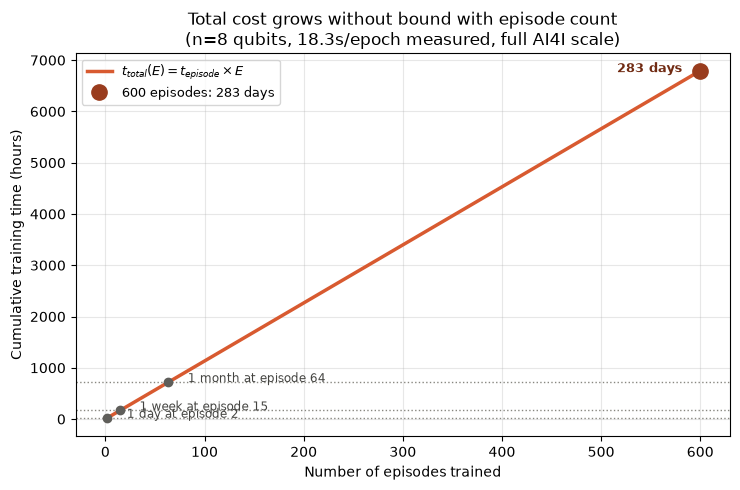
\includegraphics[width=0.75\textwidth]{figure/time_to.png}
\caption{Cumulative PennyLane training time versus episode count, built from the measured 18.3\,s/epoch figure at full-AI4I scale: 600 episodes (PPO's training length) would take approximately 283 days for a single agent.}
\label{fig:time_to_train}
\end{figure}

In practice, a result labelled ``simulate'' in this report (e.g. \Cref{tab:sim8g}) is generated entirely by the calibrated surrogate -- useful for isolating the effect of a single factor such as cost type quickly and cheaply, but not on its own a claim about the real circuit -- while a result labelled ``PennyLane'' (\Cref{tab:heart}) is the physically faithful case that the two-simulator design exists to make trainable in the first place.

\FloatBarrier
\subsubsection{Agent Design and States}
The scheduler is modelled formally as a Markov Decision Process, the tuple (S, A, P, R, $\gamma$) \citep{sutton2018reinforcement}. S is the sixteen-dimensional telemetry space described below; A is the five-action discrete space of \Cref{tab:actions}; P is the (unknown, backend-dependent) transition kernel induced by one epoch of circuit optimization under a chosen action; R is the scalar reward of Section~4.7.3; and $\gamma$ is the discount factor used by both agents to weight future epochs against the immediate one. Framing depth scheduling this way makes the problem amenable to standard policy-gradient and value-based RL methods without any quantum-specific modification to the algorithms themselves -- the quantum-specific part of the problem is entirely contained in how S, A, and R are computed from the circuit, not in how the agent is trained.

The state is a sixteen-dimensional telemetry vector summarizing the health of the circuit and its training dynamics; the most important components are listed in \Cref{tab:state}. The agent chooses among five discrete actions (\Cref{tab:actions}). Two agents are implemented and compared: a PPO actor-critic and a DQN value network. Both agents observe the identical state vector and act on the identical action space, so any difference in their behaviour reported in Section~6 is attributable to the learning algorithm rather than to a difference in what each agent is allowed to see or do.

\begin{table}[htbp]
\centering
\caption{Groups of the 16-dimensional MDP state vector (STATE\_DIM = 16).}
\label{tab:state}
\begin{tabular}{|p{3cm}|p{10cm}|}
\hline
\textbf{Group} & \textbf{Representative features} \\
\hline
Gradient health & spatial gradient variance, gradient norm, near-zero-gradient ratio \\
Training dynamics & training loss, validation loss, change in loss ($\Delta$loss) \\
Architecture & current depth, number of entangling gates, remaining depth budget \\
Diagnosis (Section~4.4.1) & solved/converged, local-minimum, dead-layer, ambiguous, and true-barren-plateau flags \\
Derived & relative weak-layer indicator (rel\_weak) and other normalized ratios \\
\hline
\end{tabular}
\end{table}

\begin{table}[htbp]
\centering
\caption{Action space (N\_ACTIONS = 5).}
\label{tab:actions}
\begin{tabular}{|p{4.5cm}|p{8.5cm}|}
\hline
\textbf{Action} & \textbf{Effect} \\
\hline
keep & Hold the current architecture and continue training. \\
add\_layer & Append a new parameterized layer (subject to the mask window). \\
propose\_prune\_layer & Soft-mask a layer for possible removal. \\
stop\_growth & Freeze the architecture for the remainder of training. \\
propose\_reduce\_entanglement & Reduce the entangling strength among gates. \\
\hline
\end{tabular}
\end{table}

\subsubsection{Reward System}
The reward combines several terms that trade off gradient health, loss improvement, and resource use. The weights actually used are given in \Cref{tab:reward}. An important and honestly-reported consequence of these weights is that the loss-improvement term (weight 5.0) dominates the gradient-variance term (weight 0.5): across the regimes reported in Section~6, this means the agent chiefly learns to optimize loss under a resource constraint rather than to avoid barren plateaus directly, and at the qubit counts evaluated here a clearly separable plateau-avoidance signal -- where growing depth is driven by low gradient variance rather than by loss alone -- has not been isolated; whether one would emerge under a local cost at a larger, currently out-of-scope qubit count (Section~1.6) is accordingly left as an open question rather than a demonstrated result.

\begin{table}[htbp]
\centering
\caption{Reward-term weights.}
\label{tab:reward}
\begin{tabular}{|p{1.5cm}|p{1.8cm}|p{9.5cm}|}
\hline
\textbf{Term} & \textbf{Weight} & \textbf{Meaning} \\
\hline
w1 & 0.5 & gradient-variance health \\
w2 & 5.0 & improvement in loss ($\Delta$loss) -- dominant term \\
w3 & 0.05 & depth / resource penalty \\
w4 & 0.02 & entangling-gate penalty \\
w5 & 1.0 & commit bonus for accepted mutations \\
w6 & 0.5 & rollback / stability shaping \\
\hline
\end{tabular}
\end{table}

\subsubsection{RL Algorithm and Training Strategy}
Two standard algorithms are used without exotic modifications. PPO \citep{schulman2017proximal} is a clipped-objective actor-critic that updates the policy conservatively; it is trained for 600 episodes. \Cref{fig:ppo_arch} shows its architecture: a shared two-layer, 128-unit MLP body (Tanh) feeds a masked 5-logit policy head and a scalar value head; each update computes a normalized GAE advantage from the stored rollout and applies the clipped surrogate objective (probability ratio clipped to $\pm20\%$) over 10 epochs of minibatch-64 backpropagation. DQN \citep{mnih2015human} is a value-based method with a target network and experience replay; it is trained for 1000 episodes. \Cref{fig:dqn_arch} shows its architecture: an online Q-network (the same two-layer, 128-unit body, ReLU instead of Tanh) outputs five Q-values; invalid actions are masked to $-\infty$ \emph{after} the network rather than inside it, transitions are pushed to a 50k-capacity replay buffer and sampled in minibatches of 64, and the target is computed Double-DQN style -- the online network selects the action, the target network evaluates it -- before a smooth-L1 TD loss updates the online network. Both use action masking so that invalid mutations (for example adding beyond the depth cap) are never selected. Proposed mutations are evaluated inside a soft-mask window and are either committed if they improve a peak-loss criterion or rolled back otherwise, which gives the agent a safe way to explore architecture changes without permanently damaging the model.

\begin{figure}[htbp]
\centering
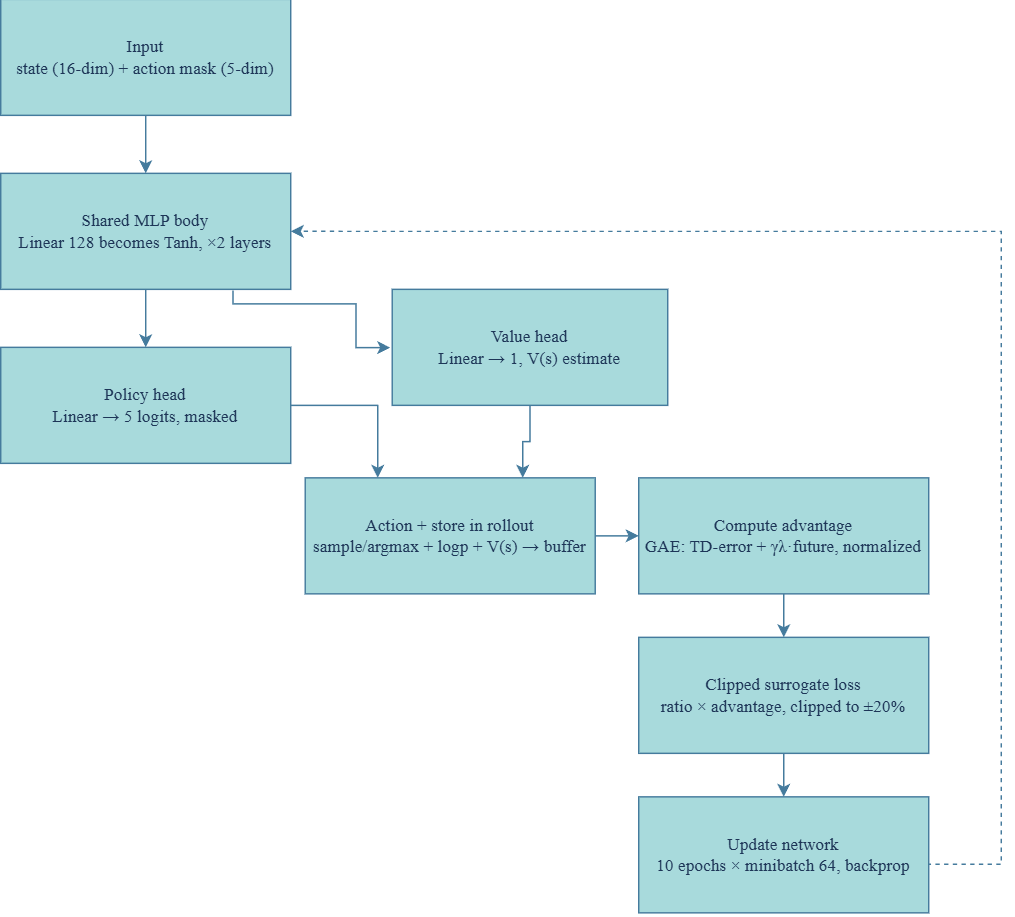
\includegraphics[width=0.7\textwidth]{figure/PPO.drawio.png}
\caption{PPO network architecture and update loop: shared MLP body, masked policy head and value head, GAE advantage estimation, and the clipped surrogate objective.}
\label{fig:ppo_arch}
\end{figure}

\begin{figure}[htbp]
\centering
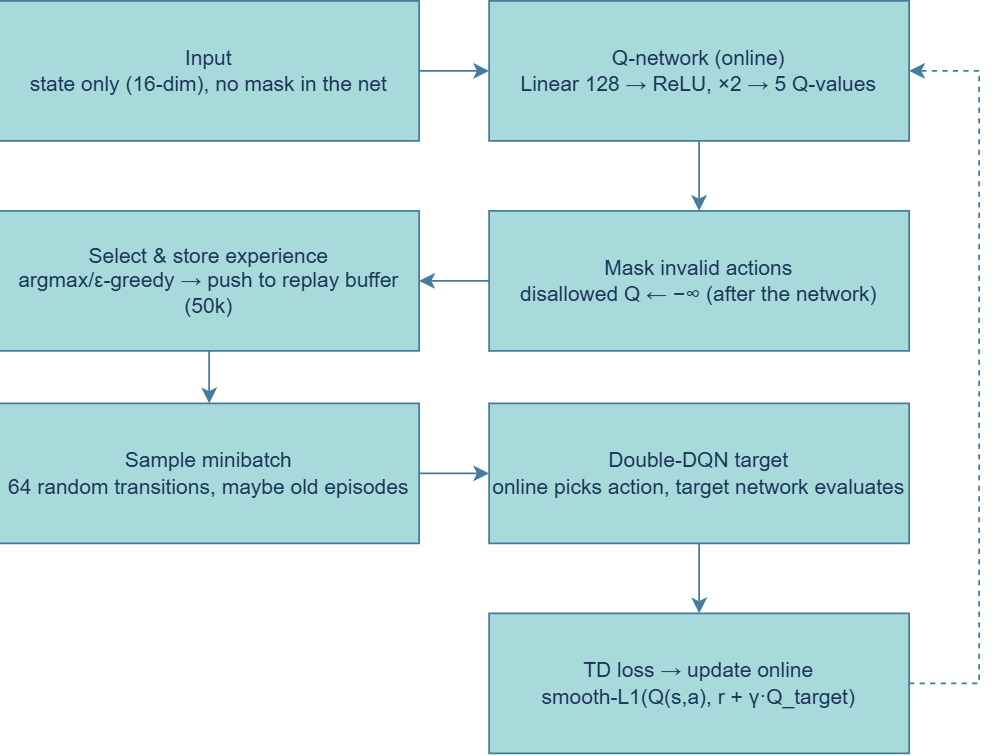
\includegraphics[width=0.7\textwidth]{figure/DQN.drawio.png}
\caption{DQN network architecture and update loop: online Q-network, post-hoc action masking, replay-buffer sampling, and the Double-DQN target used for the smooth-L1 TD update.}
\label{fig:dqn_arch}
\end{figure}

\FloatBarrier
\subsubsection{Static Baseline Schedulers}
The two static baselines that every table in Section~6 compares the learned agents against are themselves rule-based decision trees over the same telemetry and the same offline, calibrated threshold $\tau$ from the Stage~1C risk table (Section~4.7.1), not free parameters left unspecified. \Cref{fig:rule_baseline} shows the hand-tuned \textbf{Rule} scheduler: in a fixed priority order, it prunes a layer diagnosed as dead, else reduces entanglement if the gradient norm signals a global barren-plateau risk, else adds a layer while the circuit is still shallow (depth $<6$) and loss is stable, else stops growth once depth reaches 6, holding the architecture otherwise. \Cref{fig:greedy_baseline} shows the \textbf{Greedy} heuristic, the same four-branch structure with different, more aggressive thresholds: a layer is pruned once it contributes less than 15\% of the mean layer weight, entanglement is reduced once the near-zero-gradient ratio (\Cref{tab:state}) reaches 0.4, growth stops once the gradient variance has both hit its calibrated floor and fallen to or below $\tau$, and a layer is added whenever variance exceeds three times $\tau$. Both baselines are deterministic and receive no training; the only difference between them and the learned agents above is that their mapping from telemetry to action is hand-specified rather than learned from the reward of \Cref{tab:reward}.

\begin{figure}[htbp]
\centering
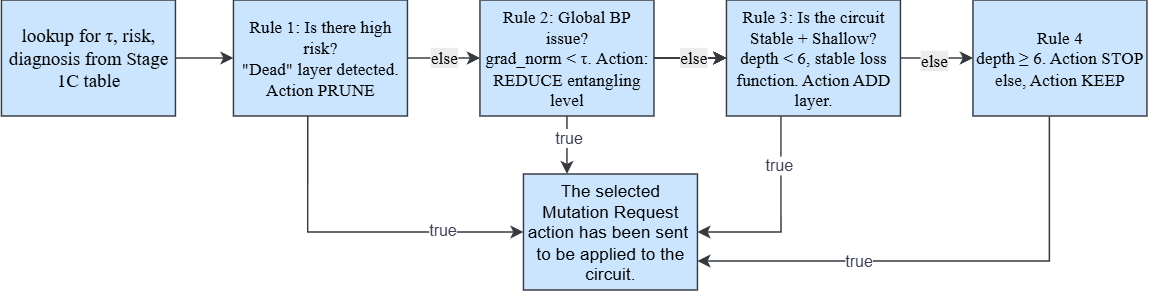
\includegraphics[width=1\textwidth]{figure/Rule.drawio.png}
\caption{Decision logic of the hand-tuned Rule baseline: a fixed priority order over dead-layer pruning, global-BP entanglement reduction, growth, and a depth-6 stop condition.}
\label{fig:rule_baseline}
\end{figure}

\begin{figure}[htbp]
\centering
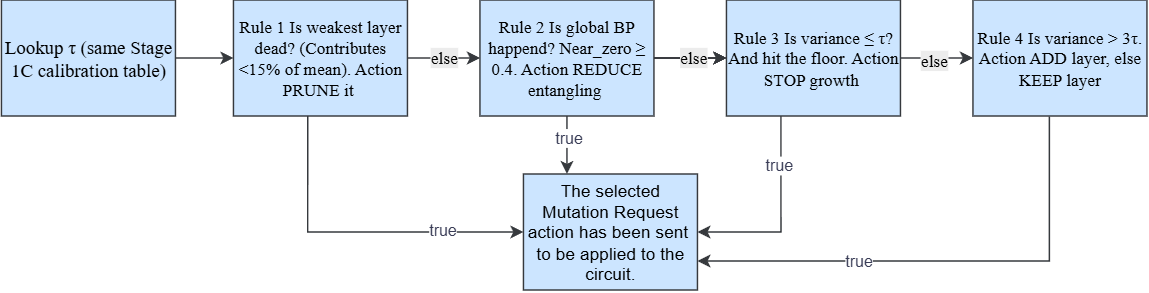
\includegraphics[width=1\textwidth]{figure/greedy.drawio.png}
\caption{Decision logic of the Greedy baseline: the same four-branch structure as the Rule baseline, with different thresholds (15\% weakest-layer contribution, 0.4 near-zero-gradient ratio, and a variance-relative-to-$\tau$ stop/grow condition).}
\label{fig:greedy_baseline}
\end{figure}

Algorithm~1 formalizes the per-epoch loop that both agents interact with, independently of which physics backend (simulate or PennyLane) is behind it. The commit/rollback guard is what allows the agent to propose a structural change to the circuit without risking the run: a proposal is only made permanent if it improves the tracked peak-loss criterion, and is otherwise reverted before the next epoch begins.

\begin{algorithm}[h]
\caption{One deployment/training epoch under the agent-controlled environment}
\label{alg:epoch}
\begin{algorithmic}[1]
\State \textbf{Input:} circuit at depth $d$, telemetry state $s_t$, peak-loss tracker $L^\star$
\State $a_t \gets \pi(s_t)$ \Comment{agent selects one of the five actions (\Cref{tab:actions})}
\If{$a_t$ proposes a structural change (add / prune / reduce-entanglement)}
    \State apply $a_t$ inside a soft-mask window (change not yet permanent)
\EndIf
\State run one epoch of parameter optimization on the (possibly masked) circuit
\State observe new loss $L_t$, gradient variance, and the rest of $s_{t+1}$
\If{$a_t$ proposed a structural change}
    \If{$L_t$ improves on $L^\star$}
        \State \textbf{commit}: make the change permanent; $L^\star \gets L_t$
    \Else
        \State \textbf{rollback}: revert to the pre-mutation architecture
    \EndIf
\EndIf
\State compute reward $r_t$ from $s_{t+1}$ (\Cref{tab:reward}) and return $(s_{t+1}, r_t)$
\end{algorithmic}
\end{algorithm}

The agent is trained entirely on the calibrated surrogate, where an episode corresponds to a full training run of the circuit under the agent's decisions. The learned policy is then deployed on the PennyLane statevector backend for 40 epochs, which is where all reported metrics are computed. During development, configurations were run with three random seeds on the AI4I dataset to characterize seed variance; the scheduler-comparison tables presented in Section~6 are run single-seed, always against the same two static baselines: a hand-tuned rule-based scheduler and a greedy heuristic.

\FloatBarrier
\subsubsection{Implementation Details}
The system is implemented in Python. Quantum circuits use PennyLane with the default statevector device and backpropagation gradients; the RL agents use PyTorch. The hardware-efficient ansatz is defined exactly once (single source of truth) and reused by the barren-plateau measurement stage and the deployment backend, so any ansatz change propagates automatically. Because full-simulator training would be prohibitively slow even at the project's 8-qubit scope (Section~1.6), the surrogate reduces RL training to roughly half an hour per agent.

\subsection{Ethical Considerations}

\subsubsection{Data Sensitivity}
Several datasets are sensitive: German Credit concerns financial creditworthiness and the medical datasets concern health status. The project uses these strictly as research benchmarks and does not deploy any model for real decisions, so the risk of biased or harmful predictions in practice does not arise here; nonetheless, class balancing and consistent preprocessing are applied so that reported accuracy is not inflated by imbalance. Because all experiments run on a simulator, there is no physical-hardware safety risk.

\subsubsection{Reproducibility and Data Honesty}
The project's overriding ethical commitment is data honesty -- every reported number is reproducible from a committed log, single-seed results are labelled as such, and unsupported performance claims were removed.


\section{System Design and Implementation}
\subsection{AI Model Integration}

\subsubsection{System Overview}
The system has three cooperating components: the variational circuit backend, the telemetry engine, and the reinforcement-learning scheduler. During a training run the backend performs one epoch of parameter optimization and exposes telemetry (gradient variance, loss, depth, and related features). The telemetry engine assembles the sixteen-dimensional state and passes it to the scheduler. The scheduler returns one of the five actions; a mutation engine applies the action to the circuit -- adding, soft-masking, or freezing layers -- under a commit/rollback guard. The loop repeats for the configured number of epochs. Algorithm~1 (Section~4.7.4) gives this loop formally; the description here focuses on which software component owns which responsibility, rather than on the control-flow logic itself.

\subsubsection{Component Responsibilities}
Each of the three components has a single, narrow responsibility, which is what allows the same scheduler and telemetry code to run unmodified against either physics backend (Section~4.7.1).

\begin{itemize}
\item Circuit backend (simulate or PennyLane): owns the quantum state, the parameter-optimization step, and the raw measurement outputs. It has no knowledge of the RL agent, the reward, or the action space; its only external contract is to accept one epoch's worth of optimization steps and return the resulting loss, accuracy, and gradient statistics.
\item Telemetry engine: owns the sixteen-dimensional state vector. It reads the raw statistics from the circuit backend, computes derived quantities ($\Delta$loss, the near-zero-gradient ratio, rel\_weak), and normalizes everything into the fixed-size vector the scheduler expects, regardless of which backend produced the raw numbers.
\item Reinforcement-learning scheduler and mutation engine: own the policy and the architecture-change logic. The scheduler consumes only the telemetry vector and returns only one of the five discrete actions (\Cref{tab:actions}); the mutation engine is the sole component permitted to modify the circuit's structure, and it does so only through the commit/rollback protocol of Algorithm~1.
\end{itemize}

\subsection{Data Flow and Processing}

\subsubsection{Preprocessing and Training Flow}
Raw data enters as CSV. The preprocessing pipeline first splits the data deterministically (by seed) into train and validation (70/30), then fits a standardization (Z-score) on the training split only, reconciles the feature count with the qubit count by PCA, one-to-one mapping, or zero-padding as appropriate (Section~4.2), and finally rescales features to the angle-encoding range [0, π]. The training split drives parameter optimization and the validation split drives the scheduler's accept/rollback decisions; the deployment and comparison scripts behind Section~6 do not additionally carve out a held-out test split (Section~4.5), though the shared loader supports one and it is used separately by the prediction-export script behind the demonstration interface (Section~5.3).

\subsubsection{Telemetry and Logging Flow}
Telemetry produced each epoch flows to the scheduler, and the resulting per-epoch record -- loss, accuracy, depth, action, commit/rollback counters -- is written to a deployment log that is the single source for every reported number.

\subsection{Deployment Strategy}

\subsubsection{Train-on-Surrogate, Deploy-on-PennyLane Workflow}
The confirmed workflow is train-on-surrogate, deploy-on-PennyLane. The RL policy is trained against the surrogate and then executed on the statevector simulator, which produces the deployment logs and the final trained circuit parameters used for inference. For the demonstration, the trained circuit is applied to held-out test samples to produce live single-sample predictions; because the parameters are captured immediately after training, no separate weight-persistence step is required for the demonstration to be reproducible.

\subsubsection{Reuse Across Experimental Regimes}
The same deployment procedure is reused, unmodified, for every regime reported in Section~6: only the four environment parameters described in Section~4.7.1 (dataset, qubit count, cost type, depth bounds) and the choice of physics backend change between the PennyLane-real run (\Cref{tab:heart}) and the simulate-backend run (\Cref{tab:sim8g}). This is a direct consequence of the component-responsibility split in Section~5.1 -- because the scheduler and telemetry engine never reference the backend directly, deploying against a new regime is a configuration change, not a code change, which is also why the regimes in Section~6 could be produced from two scripts (Appendix~C) rather than separate ones.

\subsection{Scalability and Maintenance}

\subsubsection{Scalability Axes}
The design scales along three axes. New datasets are added through a small preparation script and a single loader branch, without touching the model. New qubit counts or cost types are supported by re-calibrating the surrogate. Maintenance is simplified by the single-source-of-truth ansatz: any change to the circuit is made in one place and is automatically reflected in measurement, training, and deployment. The two-simulator split also means that expensive statevector evaluation is only incurred at deployment, keeping the iteration loop fast.

\subsubsection{Reuse in the Section 6 Sweep}
This same scalability axis is what let the Section~6.2 fixed-depth sweep be run as a batch of independent, differently-configured deployments rather than as bespoke code: the cost-type sweep is, mechanically, the same re-calibration-then-deploy procedure used for any other configuration change, repeated six times per regime for k = 2, 4, 6, 8, 12, 16. The maintenance cost of adding a new regime to Section~6 is therefore one surrogate re-calibration and one deployment run, not a new code path.


\section{Results and Discussion}
\subsection{Results and Analysis}

\subsubsection{Barren-Plateau Scaling}
\textbf{[PENDING re-measurement -- see note below.]} The gradient variance measured on the AI4I 2020 predictive-maintenance dataset (the project's primary dataset; see Section~4.2) was previously reported as dropping by a factor of 57.3$\times$ from 6 to 12 qubits, close to the theoretical $2^{-n}$ expectation. That specific comparison is now out of scope: the project's validated qubit range on available hardware is $n\le8$ (Section~1.6), so the scaling claim needs to be re-measured over 6 to 8 qubits, where the theoretical $2^{-n}$ expectation is a much smaller $4\times$ drop rather than $64\times$ -- a genuinely weaker signal that has not yet been confirmed empirically at this narrower range. \Cref{tab:ai4i} below is pending the same re-scoped re-run, together with the SMOTE-related data-pipeline correction noted after it.

\begin{table}[htbp]
\centering
\caption{Scheduler comparison on AI4I (n = 8, local cost, mean over 3 seeds) -- pending re-run.}
\label{tab:ai4i}
\begin{tabular}{|p{3cm}|p{2cm}|p{2.3cm}|p{2cm}|p{2.5cm}|}
\hline
\textbf{Scheduler} & \textbf{Type} & \textbf{Accuracy} & \textbf{F1} & \textbf{Depth} \\
\hline
Rule & static & -- & -- & -- \\
Greedy & static & -- & -- & -- \\
PPO & learned & -- & -- & -- \\
DQN & learned & -- & -- & -- \\
\hline
\end{tabular}
\end{table}

\textbf{Data-pipeline and scope note.} This table previously reported $n=12$ results generated before two subsequent changes: (i) the qubit range validated on available hardware was narrowed to $n\le8$ (Section~1.6, RAM/runtime cost of PennyLane statevector simulation), which alone requires this benchmark to move from $n=12$ to $n=8$; and (ii) the AI4I loader was changed from forcing a 339/339 undersampled split to preserving the natural $\approx$3.4\% class imbalance and correcting it with SMOTE on the training split only (Section~4.2, AI4I 2020 Predictive Maintenance). Both changes require the primary benchmark to be re-run at $n=8$ against the corrected loader before this table can be filled in; the old $n=12$ numbers have been removed rather than left in place mislabelled as $n=8$.

\subsubsection{Primary AI4I Benchmark}
\textbf{[PENDING -- to be written once \Cref{tab:ai4i} is re-run at $n=8$; see note above.]}

\subsubsection{Real Deployment versus a Synthetic Comparison}
Beyond the primary AI4I evaluation above, a second block of results combines one real deployment on an independent dataset with a synthetic comparison at the same qubit count. \Cref{tab:heart} is the real, physical anchor: the policy deployed on the actual PennyLane statevector circuit for Heart Disease at 8 qubits under a local cost. \Cref{tab:sim8g} varies only the cost type (global instead of local) at the same 8-qubit count on synthetic data, isolating the effect of cost type on trainability and scheduler behaviour while holding qubit count fixed; because the cost type and dataset differ between these two tables, they should be read as separate regimes rather than as a single matched comparison.

\begin{table}[htbp]
\centering
\caption{Scheduler comparison -- PennyLane real deployment (Heart Disease, n = 8 qubits, local cost, single seed).}
\label{tab:heart}
\begin{tabular}{|p{3cm}|p{2cm}|p{2.3cm}|p{2cm}|p{2.5cm}|}
\hline
\textbf{Scheduler} & \textbf{Type} & \textbf{Accuracy} & \textbf{F1} & \textbf{Depth} \\
\hline
Rule & static & 0.518 & 0.608 & 4 \\
Greedy & static & 0.807 & 0.795 & 16 \\
PPO & learned & 0.735 & 0.703 & 2 \\
DQN & learned & 0.554 & 0.667 & 2 \\
\hline
\end{tabular}
\end{table}

\subsubsection{PennyLane Real Deployment (Heart Disease)}
On the real PennyLane deployment on Heart Disease at 8 qubits with a local cost, the greedy heuristic achieves the best accuracy (0.807) and F1 (0.795), growing the circuit to depth 16; the fixed-depth baselines at k = 8 and k = 16 perform almost identically (accuracy 0.795), showing that once the circuit is deep enough under a local cost the gradient remains trainable and extra depth adds little further benefit. PPO matches a shallow fixed-depth baseline (accuracy 0.735 at depth 2) without growing the circuit, while the hand-tuned rule and DQN both underperform, with DQN in particular collapsing to a near-chance ROC AUC (0.492). The ranking Greedy > PPO > Rule > DQN on this real, trainable deployment is a useful counterexample to any claim that one scheduler dominates universally.

\begin{table}[htbp]
\centering
\caption{Scheduler comparison -- simulated deployment (synthetic data, n = 8 qubits, global cost, single seed).}
\label{tab:sim8g}
\begin{tabular}{|p{3cm}|p{2cm}|p{2.3cm}|p{2cm}|p{2.5cm}|}
\hline
\textbf{Scheduler} & \textbf{Type} & \textbf{Accuracy} & \textbf{F1} & \textbf{Depth} \\
\hline
Rule & static & 0.680 & 0.666 & 6 \\
Greedy & static & 0.908 & 0.889 & 16 \\
PPO & learned & 0.735 & 0.720 & 7 \\
DQN & learned & 0.680 & 0.666 & 6 \\
\hline
\end{tabular}
\end{table}

\subsubsection{Same-Qubit-Count Synthetic Comparison (Global Cost)}
At the same qubit count as the real deployment (8) but with a global cost, the synthetic run shows the same qualitative ranking as \Cref{tab:heart} -- greedy on top (0.908), PPO next (0.735) -- but with higher absolute accuracy across the board. DQN and the hand-tuned rule land on an identical accuracy (0.680) at the same depth (6), an exact tie that is a coincidence of this single seed rather than a general result. The qualitative agreement with the real \Cref{tab:heart} ranking is reassuring for the synthetic pipeline, but the different cost type (global vs local) means the gap in absolute accuracy should not be over-interpreted.

\subsubsection{Additional Single-Dataset Deployments (German Credit, Parkinson's, Pima)}
Beyond the core evaluation design above, the project also logged one real PennyLane deployment run (8 qubits, single seed) on each of three secondary datasets from \Cref{tab:datasets} -- German Credit, Parkinson's, and Pima -- using the same rule/greedy/PPO/DQN comparison procedure as \Cref{tab:heart}. These were exploratory checks rather than part of the core evaluation design (Section~1.4), and a separate run-configuration file was not retained alongside the logs, so the cost type and seed are inferred from the comparison pipeline's default configuration (local cost, seed 123) rather than confirmed from a recorded config; they are reported here, with that caveat, because the logs already exist and were otherwise undocumented.

\begin{table}[htbp]
\centering
\caption{Scheduler comparison -- PennyLane real deployment (German Credit, n = 8 qubits, single seed; cost type inferred as local from the pipeline default).}
\label{tab:german}
\begin{tabular}{|p{3cm}|p{2cm}|p{2.3cm}|p{2cm}|p{2.5cm}|}
\hline
\textbf{Scheduler} & \textbf{Type} & \textbf{Accuracy} & \textbf{F1} & \textbf{Depth} \\
\hline
Rule & static & 0.706 & 0.640 & 6 \\
Greedy & static & 0.667 & 0.706 & 3 \\
PPO & learned & 0.722 & 0.734 & 6 \\
DQN & learned & 0.628 & 0.511 & 1 \\
\hline
\end{tabular}
\end{table}

On German Credit, PPO attains the best accuracy (0.722) and F1 (0.734) of the four schedulers, narrowly ahead of the hand-tuned rule (0.706 accuracy) at the same committed depth (6); greedy stops early at depth 3, and DQN collapses to depth 1 with the weakest F1 (0.511). This is the one regime in this report where PPO outright wins -- a useful reminder that the ranking between the rule and PPO is not fixed across datasets, to be checked against the re-run AI4I benchmark (\Cref{tab:ai4i}) once available.

\begin{table}[htbp]
\centering
\caption{Scheduler comparison -- PennyLane real deployment (Parkinson's, n = 8 qubits, single seed; cost type inferred as local from the pipeline default).}
\label{tab:parkinsons}
\begin{tabular}{|p{3cm}|p{2cm}|p{2.3cm}|p{2cm}|p{2.5cm}|}
\hline
\textbf{Scheduler} & \textbf{Type} & \textbf{Accuracy} & \textbf{F1} & \textbf{Depth} \\
\hline
Rule & static & 0.899 & 0.892 & 6 \\
Greedy & static & 0.843 & 0.851 & 8 \\
PPO & learned & 0.730 & 0.745 & 7 \\
DQN & learned & 0.640 & 0.515 & 2 \\
\hline
\end{tabular}
\end{table}

On Parkinson's, the hand-tuned rule is clearly the strongest scheduler (0.899 accuracy, 0.892 F1), with greedy second; both static schedulers beat PPO and DQN by a wide margin. DQN is notably worse than its own 0.719 starting accuracy (\texttt{acc\_start} in the underlying log), meaning the agent's depth decisions actively hurt this small, 96-sample dataset rather than merely failing to help -- another instance of the DQN instability already seen on \Cref{tab:heart}.

\begin{table}[htbp]
\centering
\caption{Scheduler comparison -- PennyLane real deployment (Pima, n = 8 qubits, single seed; cost type inferred as local from the pipeline default).}
\label{tab:pima}
\begin{tabular}{|p{3cm}|p{2cm}|p{2.3cm}|p{2cm}|p{2.5cm}|}
\hline
\textbf{Scheduler} & \textbf{Type} & \textbf{Accuracy} & \textbf{F1} & \textbf{Depth} \\
\hline
Rule & static & 0.689 & 0.680 & 6 \\
Greedy & static & 0.714 & 0.742 & 8 \\
PPO & learned & 0.578 & 0.558 & 2 \\
DQN & learned & 0.708 & 0.704 & 2 \\
\hline
\end{tabular}
\end{table}

On Pima, greedy is best (0.714 accuracy), with DQN a close second (0.708) despite committing to a much shallower depth (2 versus greedy's 8); PPO is the weakest scheduler here and, as on Parkinson's, ends below its own starting accuracy (0.590), indicating an unproductive depth change rather than a neutral one. Across all three supplementary datasets, no single scheduler wins twice: PPO wins on German Credit, the rule wins on Parkinson's, and greedy wins on Pima. This adds three more data points to the same conclusion the core evaluation reaches -- that scheduler ranking is regime- and dataset-dependent -- while underscoring, precisely because these three runs are single-seed and only single-dataset checks, that they should be read as corroborating evidence rather than as an independent, equally-weighted evaluation alongside \Cref{tab:ai4i,tab:heart,tab:sim8g}.

\subsection{Extended Fixed-Depth Sweep}

\subsubsection{Sweep Methodology}
\Cref{tab:ai4i,tab:heart,tab:sim8g} summarize each regime with only four schedulers (Rule, Greedy, PPO, DQN) for readability. The deployment pipeline, however, also runs a dense fixed-depth sweep (k = 2, 4, 6, 8, 12, 16) as a reference curve against which the adaptive schedulers can be judged: if a learned or hand-tuned scheduler settles on a depth d, this sweep tells us whether d was actually close to the accuracy-maximizing depth for that regime, or whether the scheduler stopped short (or overshot). This subsection reports the full sweep for the two single-seed experimental configurations behind \Cref{tab:heart,tab:sim8g}, so that those summary rankings can be checked against the underlying accuracy-vs-depth curve rather than taken on faith; the three-seed primary AI4I benchmark (\Cref{tab:ai4i}) is a separate, higher-cost run and was not additionally swept across depths.


\begin{table}[htbp]
\centering
\caption{Fixed-depth sweep -- PennyLane real deployment (Heart Disease, n = 8 qubits, local cost).}
\label{tab:sweep_heart}
\begin{tabular}{|p{2.4cm}|p{2.3cm}|p{2cm}|p{2.4cm}|}
\hline
\textbf{Depth k} & \textbf{Accuracy} & \textbf{F1} & \textbf{ROC AUC} \\
\hline
2 & 0.735 & 0.703 & 0.835 \\
4 & 0.759 & 0.756 & 0.845 \\
8 & 0.795 & 0.790 & 0.866 \\
16 & 0.795 & 0.790 & 0.876 \\
\hline
\end{tabular}
\end{table}

\subsubsection{Heart Disease Sweep (Real Deployment)}
On the real Heart Disease deployment, accuracy rises steeply from depth 2 to depth 4 (+0.024) and then flattens almost completely between depth 8 and depth 16 (+0.000 accuracy, +0.010 ROC AUC), consistent with the local-cost gradient-variance measurement in Section~6.1: once the circuit is deep enough for the local cost to keep gradients alive, additional depth buys almost nothing. This is exactly why Greedy (which grows to depth 16 by construction) and the k = 8 fixed baseline land within 0.4 percentage points of each other -- the accuracy-maximizing depth on this real circuit is reached well before the depth cap, and the fixed-depth curve is the evidence, not just the scheduler comparison in \Cref{tab:heart}.

\begin{table}[htbp]
\centering
\caption{Fixed-depth sweep -- simulated deployment (synthetic, n = 8 qubits, global cost).}
\label{tab:sweep_sim8g}
\begin{tabular}{|p{2.4cm}|p{2.3cm}|p{2cm}|p{2.4cm}|}
\hline
\textbf{Depth k} & \textbf{Accuracy} & \textbf{F1} & \textbf{ROC AUC} \\
\hline
2 & 0.254 & 0.249 & 0.627 \\
4 & 0.519 & 0.509 & 0.760 \\
6 & 0.680 & 0.666 & 0.840 \\
8 & 0.777 & 0.762 & 0.889 \\
12 & 0.873 & 0.855 & 0.936 \\
16 & 0.453 & 0.444 & 0.727 \\
\hline
\end{tabular}
\end{table}

\subsubsection{Synthetic 8-Qubit Global-Cost Sweep}
The synthetic q = 8, global-cost sweep is monotonically increasing from depth 2 through depth 12, gaining roughly 0.10--0.15 accuracy per doubling of depth, before dropping sharply at depth 16 (accuracy falls from 0.873 at k = 12 to 0.453 at k = 16). This non-monotonic tail is a single-seed artefact of the calibrated surrogate rather than a physical prediction -- it is precisely the kind of extrapolation risk flagged in Section~4.7.1, where the surrogate is described as reliable only within its calibrated regime. It also explains why Greedy, which happens to land on depth 16 in \Cref{tab:sim8g}, still reports a high accuracy (0.908): Greedy's own trajectory through the depth-vs-accuracy landscape does not pass through the same point as this independently swept curve, since the two runs commit layers under different stopping criteria. The practical lesson is that a single fixed-depth sweep on a single seed should not be read as a precise accuracy-vs-depth function, only as a rough guide to where the trainable region lies.

\subsection{Discussion}

\subsubsection{Answering the Central Research Question}
\textbf{[PENDING -- to be finalized once the AI4I n=8 benchmark is available; see note below.]} The central research question -- whether an RL agent can schedule circuit depth to keep a variational classifier trainable -- is answered with a qualified yes, though the strength of that answer depends heavily on regime rather than on the agent alone. On the real Heart Disease deployment (\Cref{tab:heart}) and its synthetic same-qubit counterpart (\Cref{tab:sim8g}), both under cost regimes where gradients stay alive, static heuristics -- greedy in particular -- match or beat the learned agents; PPO tracks a shallow fixed-depth baseline instead of demonstrating a clear advantage from adaptive growth. The clearest case for adaptive scheduling in this report is instead the supplementary German Credit deployment (\Cref{tab:german}, Section~6.1), where PPO outright wins on both accuracy and F1 -- though that result is single-seed and exploratory rather than part of the core design. This is broadly consistent with the reward analysis: because the loss-improvement weight dominates the gradient-variance weight (\Cref{tab:reward}), the agent primarily learns to optimize loss under a resource constraint rather than to actively avoid barren plateaus, so a genuine plateau-avoidance advantage is the exception here rather than the rule. \textbf{Note:} an earlier version of this section additionally reported a 20-qubit, local-cost synthetic regime in which PPO was the clear winner; that regime has been removed because it falls outside the $\le$8-qubit scope validated on available hardware (Section~1.6, RAM/runtime cost of PennyLane statevector simulation), and this paragraph should be revisited once the new AI4I n=8 benchmark (\Cref{tab:ai4i}) is available, since it is the most likely remaining source of a clear scheduler-value result.

\subsubsection{Alignment with Theory}
These findings align with the theory: local cost functions are known to weaken barren plateaus while introducing depth dependence, which is the condition under which the scheduler's depth control has the potential to matter. The honest conclusion is not that reinforcement learning is a universal remedy, but that any advantage it offers is regime-specific and modest at the qubit counts evaluated here -- and that a strong static baseline must always be reported alongside it.

\subsubsection{Limitations Encountered}
Limitations encountered during the project include the instability of single-seed deployment -- \Cref{tab:heart,tab:sim8g} above each report a single seed, so headline numbers such as greedy's 0.807 accuracy on Heart Disease (\Cref{tab:heart}) should be read as illustrative rather than statistically robust; \Cref{tab:ai4i} (AI4I) is the only three-seed result in this section, and even that is limited to a single dataset and qubit count -- together with the cost of statevector evaluation and the sensitivity of results to preprocessing choices, which motivated the standardized fit-on-train pipeline.

\subsection{Recommendations}

\subsubsection{Scheduling and Evaluation Practice}
\begin{itemize}
\item Always report a hand-tuned rule and a greedy heuristic alongside the learned scheduler; adaptive scheduling should be claimed only where it demonstrably separates from them.
\item Evaluate every headline number with at least three seeds and report mean $\pm$ standard deviation; treat single-seed runs as exploratory.
\end{itemize}

\subsubsection{Regime Selection and Simulator Fidelity}
\begin{itemize}
\item Target the local-cost regime when depth scheduling is the goal, since that is where the plateau -- and therefore the potential benefit -- is depth-dependent rather than fixed.
\item Re-calibrate the surrogate whenever the ansatz or preprocessing changes, to keep the training environment faithful to deployment.
\end{itemize}


\section{Conclusion}
\subsection{Summary of Findings}

\subsubsection{Empirical Confirmation of the Barren Plateau}
\textbf{[PENDING -- to be finalized once the AI4I n=8 benchmark is available; see Section~6.1.]} This project designed, implemented, and evaluated AL-QNN, a variational quantum classifier whose depth is scheduled online by a reinforcement-learning agent, validated at up to 8 qubits on the hardware available to the team (Section~1.6). An earlier draft of this section reported a barren-plateau confirmation on the qubit axis and a primary AI4I benchmark measured at 12 qubits; both have been withdrawn because they fall outside the project's 8-qubit scope and, independently, because the AI4I data loader has since been corrected (Section~6.1). They are pending re-measurement within the 8-qubit range.

\subsubsection{Scheduler Performance Across Regimes}
\textbf{[PENDING -- see note above; this section's strongest supporting evidence, a 20-qubit local-cost regime, has been removed as out of scope.]} Under regimes where gradients are already healthy (\Cref{tab:heart,tab:sim8g}) a static heuristic -- greedy -- matches or beats the learned agents, with PPO tracking a shallow fixed-depth baseline rather than showing a clear advantage. The one regime in this report where the learned scheduler outright wins is the supplementary German Credit deployment (\Cref{tab:german}, single-seed, Section~6.1). The learned scheduler is therefore not shown to be universally superior at the qubit counts evaluated here; whether it separates from static baselines more clearly at $n=8$ on the primary AI4I benchmark is the open question this section will answer once \Cref{tab:ai4i} is re-run.

\subsection{Contributions and Reflections on the Project}

\subsubsection{Contributions}
The project contributes: (i) a telemetry-driven MDP formulation of quantum-circuit depth scheduling with a sixteen-dimensional state and a five-action space; (ii) a practical two-simulator architecture (surrogate for training, PennyLane for deployment) that makes RL training tractable for quantum circuits; (iii) an evenhanded, multi-regime evaluation that identifies the conditions in which adaptive scheduling is worthwhile; and (iv) a reproducible, log-backed methodology.

\subsubsection{Reflections on the Process}
Reflecting on the process, the two-simulator design and the single-source-of-truth ansatz were the decisions that most improved both speed and correctness, while the main difficulty was resisting overclaiming from unstable single-seed runs.

\subsection{Threats to Validity}
Four factors limit how far the conclusions in Section~6 generalize, and are stated here explicitly rather than left implicit.

\subsubsection{Single-Seed Variance (Internal Validity)}
The primary AI4I benchmark (\Cref{tab:ai4i}) is the only three-seed table in Section~6, pending re-run at $n=8$; every other scheduler-comparison table in Section~6 is a single run. The extended fixed-depth sweep (Section~6.2) shows at least one clearly non-monotonic curve (the synthetic q = 8, global-cost regime), which is direct evidence that single-seed numbers can and do contain noise large enough to change which depth looks best; the same could in principle be true of any single headline accuracy figure elsewhere in the report.

\subsubsection{No Held-Out Test Split (Construct Validity)}
The deployment and comparison scripts behind every table in Section~6 split each dataset into a 70/30 train/validation partition only, with no separate held-out test set (Section~4.5); every reported accuracy, F1, and ROC AUC figure is therefore a validation-split metric, computed on the same data the scheduler observes every epoch to make its accept/rollback decisions. This is not a data-leakage bug -- no scaler, PCA, or model parameter is ever fit on this split -- but it does mean the reported numbers should be read as in-loop validation performance rather than performance on data the pipeline never touched, and absolute accuracy figures may carry a mild optimistic bias relative to a true held-out test set.

\subsubsection{Surrogate Fidelity (Construct Validity)}
Every ``simulate''-labelled result is generated by a classical surrogate calibrated on a limited set of real measurements (Section~4.7.1); its trends are reliable within the calibrated regime but are not a guarantee of behaviour on the real circuit outside it, which is precisely why the PennyLane-real \Cref{tab:heart} is retained as an independent anchor rather than being replaced by a cheaper synthetic equivalent.

\subsubsection{Regime Coverage (External Validity)}
All reported regimes sit at a single qubit count ($n=8$), the ceiling validated on available hardware (Section~1.6); within that fixed qubit count, two cost types (local and global) are compared, supplemented by three single-seed real deployments on other datasets (German Credit, Parkinson's, Pima; Section~6.1) reported for completeness rather than as additional matched regimes. This isolates the cost-type factor but says nothing about how either scheduler's advantage would change at a higher qubit count, since that axis was cut from the study entirely rather than sampled; the recommendations in Section~6.4 should be read as guidance for where to look next, not as a closed characterization of the full regime space, and any claim about qubit-count scaling beyond $n=8$ is outside what this report can support.

\subsection{Limitations and Future Work}
The principal limitations are that results are obtained on a noiseless simulator rather than physical hardware, that evaluation was capped at 8 qubits by the RAM and runtime cost of PennyLane statevector simulation on available hardware (Section~1.6), and that several secondary results are reported with a single seed. The most immediate item of future work is completing the AI4I benchmark at $n=8$ (\Cref{tab:ai4i}) and the corresponding barren-plateau scaling measurement, both currently pending (Section~6.1); beyond that, the most important item is to complete multi-seed runs for every regime so that the cross-regime claims can be stated with confidence intervals, and, hardware permitting, to extend the qubit range past 8 to test whether the cost-type effect observed here strengthens at larger qubit counts.



\section{Appendices}
This appendix lists the source files, log schema, and key scripts underlying the tables in Section~6, so that a reported number can be traced back to a specific run in the project repository. One exception is noted explicitly below (\Cref{tab:ai4i}) rather than left implicit.

\textbf{A. Source files for \Cref{tab:heart,tab:sim8g}.} \\
\Cref{tab:heart}: \texttt{outputs/comparison/pennylane/comparison.csv} (PennyLane, real deployment, dataset = heart, n\_qubits = 8, cost\_type = local). \\
\Cref{tab:sim8g}: \texttt{outputs/comparison/simulate\_bp\_heavy\_q8\_v2/comparison.csv} (simulate backend, synthetic, n\_qubits = 8, cost\_type = global).

\textbf{A.0 \Cref{tab:ai4i} (primary AI4I benchmark, three seeds) -- pending re-run.} This table is currently empty pending a re-run at $n=8$ (Section~6.1, Data-pipeline and scope note); once re-run, its source file should be listed here in the same format as A and A.1. For the record, the withdrawn $n=12$ version's per-seed run logs were also not locatable in the repository under a clearly matching name -- most likely overwritten by later reruns of the same comparison script during development -- so that version could never have been fully re-traced to a single committed file even before it was withdrawn for being out of the project's 8-qubit scope.

\textbf{A.1 Source files for the supplementary deployments (\Cref{tab:german,tab:parkinsons,tab:pima}, Section~6.1).} \\
\Cref{tab:german}: \texttt{outputs/comparison/german\_credit\_8q/german\_credit\_8q/comparison/comparison.csv} (PennyLane, real deployment, dataset = german\_credit, n\_qubits = 8, seed = 123; no separate run-configuration file was retained, so cost\_type is inferred as local from the comparison pipeline's default). \\
\Cref{tab:parkinsons}: \texttt{outputs/comparison/parkinsons\_8q/parkinsons\_8q/comparison/comparison.csv} (same caveat: PennyLane, real deployment, dataset = parkinsons, n\_qubits = 8, seed = 123, cost\_type inferred as local). \\
\Cref{tab:pima}: \texttt{outputs/comparison/pima\_8q\_pennylane/pima\_8q\_pennylane/comparison.csv} (same caveat: PennyLane, real deployment, dataset = pima, n\_qubits = 8, seed = 123, cost\_type inferred as local).

\textbf{B. Deployment log schema.} Each \texttt{comparison.csv} and \texttt{deploy\_log\_*.csv} file shares the same columns: \texttt{scheduler, backend, seed, epochs, acc\_start, acc\_end, acc\_delta, f1\_end, roc\_auc\_end, depth\_start, depth\_end, n\_commits, n\_rollbacks, act\_keep, act\_add\_layer, act\_stop\_growth, act\_propose\_prune\_layer, act\_propose\_reduce\_entanglement} -- the same fields referenced throughout Section~6.

\textbf{C. Key scripts.} \texttt{scripts/04\_train\_rl\_scheduler.py} trains the PPO/DQN scheduler on the calibrated surrogate and deploys the learned policy on PennyLane; \texttt{scripts/05\_compare\_schedulers.py} runs the rule, greedy, fixed-depth, PPO, and DQN schedulers under a given dataset/qubit-count/cost-type configuration and writes the corresponding \texttt{comparison.csv}; \texttt{scripts/06\_calibrate\_surrogate.py} fits the loss-floor and gradient-variance surrogate used by the simulate backend (Section~4.7.1) from the Stage 1 measurements.

\textbf{D. Repository.} All logs, scripts, and figures referenced above are tracked in the project repository described in Section~2.1.3; every number reported in this document, other than \Cref{tab:ai4i} (pending re-run, A.0) and the barren-plateau scaling figures it depends on, traces to a committed file at that location. Flagging that gap explicitly, rather than silently letting the general claim stand or backfilling it with unverified numbers, is itself an application of the data-honesty principle stated in Section~2.2.3.



\clearpage
\addcontentsline{toc}{section}{References}
\setstretch{2} %\doublespacing  %
\bibliographystyle{elsarticle-num-names}
\bibliography{refs}

\end{document}
